\subsection[Installazione]{Installazione}

\pgfdeclareimage[width=5cm]{eclipselogo}{img/eclipselogo.png}
\begin{frame}{Eclipse (I)}

  Eclipse è un \textbf{ambiente di sviluppo integrato} (\emph{IDE}) multi-linguaggio e multipiattaforma.
  \begin{center}
    \pgfuseimage{eclipselogo}
  \end{center}

\end{frame}

\begin{frame}{Eclipse (II)}

  Eclipse è un \textbf{ambiente di sviluppo integrato} (\emph{IDE}) multi-linguaggio e multipiattaforma.
  
  \begin{itemize}
    \item software \textbf{libero} e \textbf{open source};
    \item versione 1.0 rilasciata nel 2001, versione stabile 4.5.0 \emph{Mars} (giugno 2015), voi avete 4.4.0 \emph{Luna};
    \item multipiattaforma;
    \item estendibile con \textbf{plugins};
  \end{itemize}
\end{frame}

\begin{frame}{Scaricare e installare Eclipse}

  \begin{enumerate}
    \item Scaricare Java \textbf{JDK} (\emph{Java Development Kit}) \url{http://www.oracle.com/technetwork/java/javase/downloads/index.html};
    \item Scaricare Eclipse \url{https://www.eclipse.org/downloads/};
    \begin{itemize}
      \item \url{https://www.cs.umd.edu/eclipse/}
    \end{itemize}
  \end{enumerate}
\end{frame}

\begin{frame}{Verificare che l'installazione di Java è andata a buon fine}

  Aprendo un \textbf{terminale} (o \emph{shell}) (*nix) o ``prompt dei comandi'' (Windows): \newline
  \texttt{
     \$ java -version \newline                                                                                                          
     java version "1.8.0\_60" \newline
     Java(TM) SE Runtime Environment (build 1.8.0\_60-b27) \newline
     Java HotSpot(TM) 64-Bit Server VM (build 25.60-b23, mixed mode)
     }

\end{frame}
 

\begin{frame}{Altre IDE}

  Esistono molte altre IDE:
  \begin{enumerate}
    \item \textbf{NetBeans}: \url{https://netbeans.org/}
    \item \textbf{IntelliJ IDEA}: \url{https://www.jetbrains.com/idea/}
  \end{enumerate}
\end{frame}
 
\subsection[Creazione progetto]{Creazione progetto}

\pgfdeclareimage[width=6cm]{eclipse_splash}{img/eclipse/eclipse_mars_splash_screen.png}
\begin{frame}{Avvio di Eclipse (I)}
  \begin{center}
    \pgfuseimage{eclipse_splash}
  \end{center}
\end{frame}

\pgfdeclareimage[width=6cm]{workspace}{img/eclipse/workspace.png}
\begin{frame}{Workspace}
  \textbf{Workspace}:
  \begin{center}
    \pgfuseimage{workspace}
  \end{center}
\end{frame}
% {
%   \setbeamercolor{background canvas}{bg=}
%   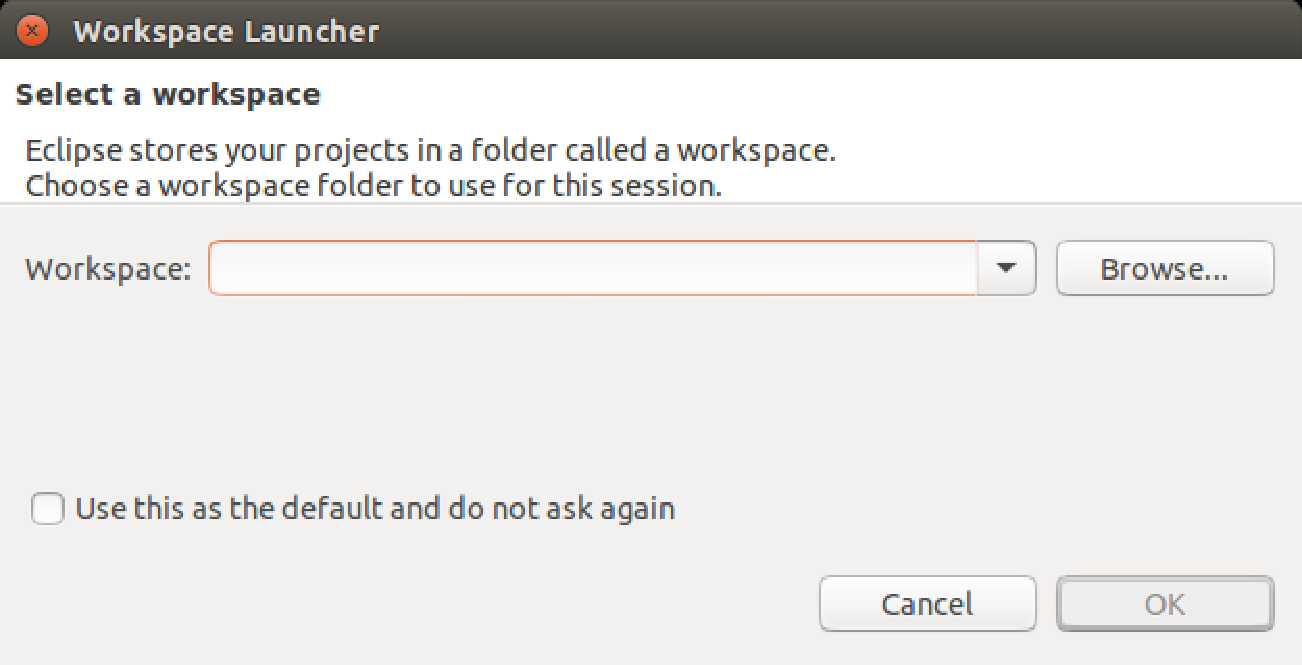
\includepdf[pages={1}]{img/eclipse/workspace.pdf}
% }

% \pgfdeclareimage[height=\paperheight,width=\paperwidth]{welcome}{img/eclipse/welcome.png}
% \begin{frame}{Avvio di Eclipse}
%   \begin{center}
%     \pgfuseimage{welcome}
%   \end{center}
% \end{frame}
{
  \setbeamercolor{background canvas}{bg=}
  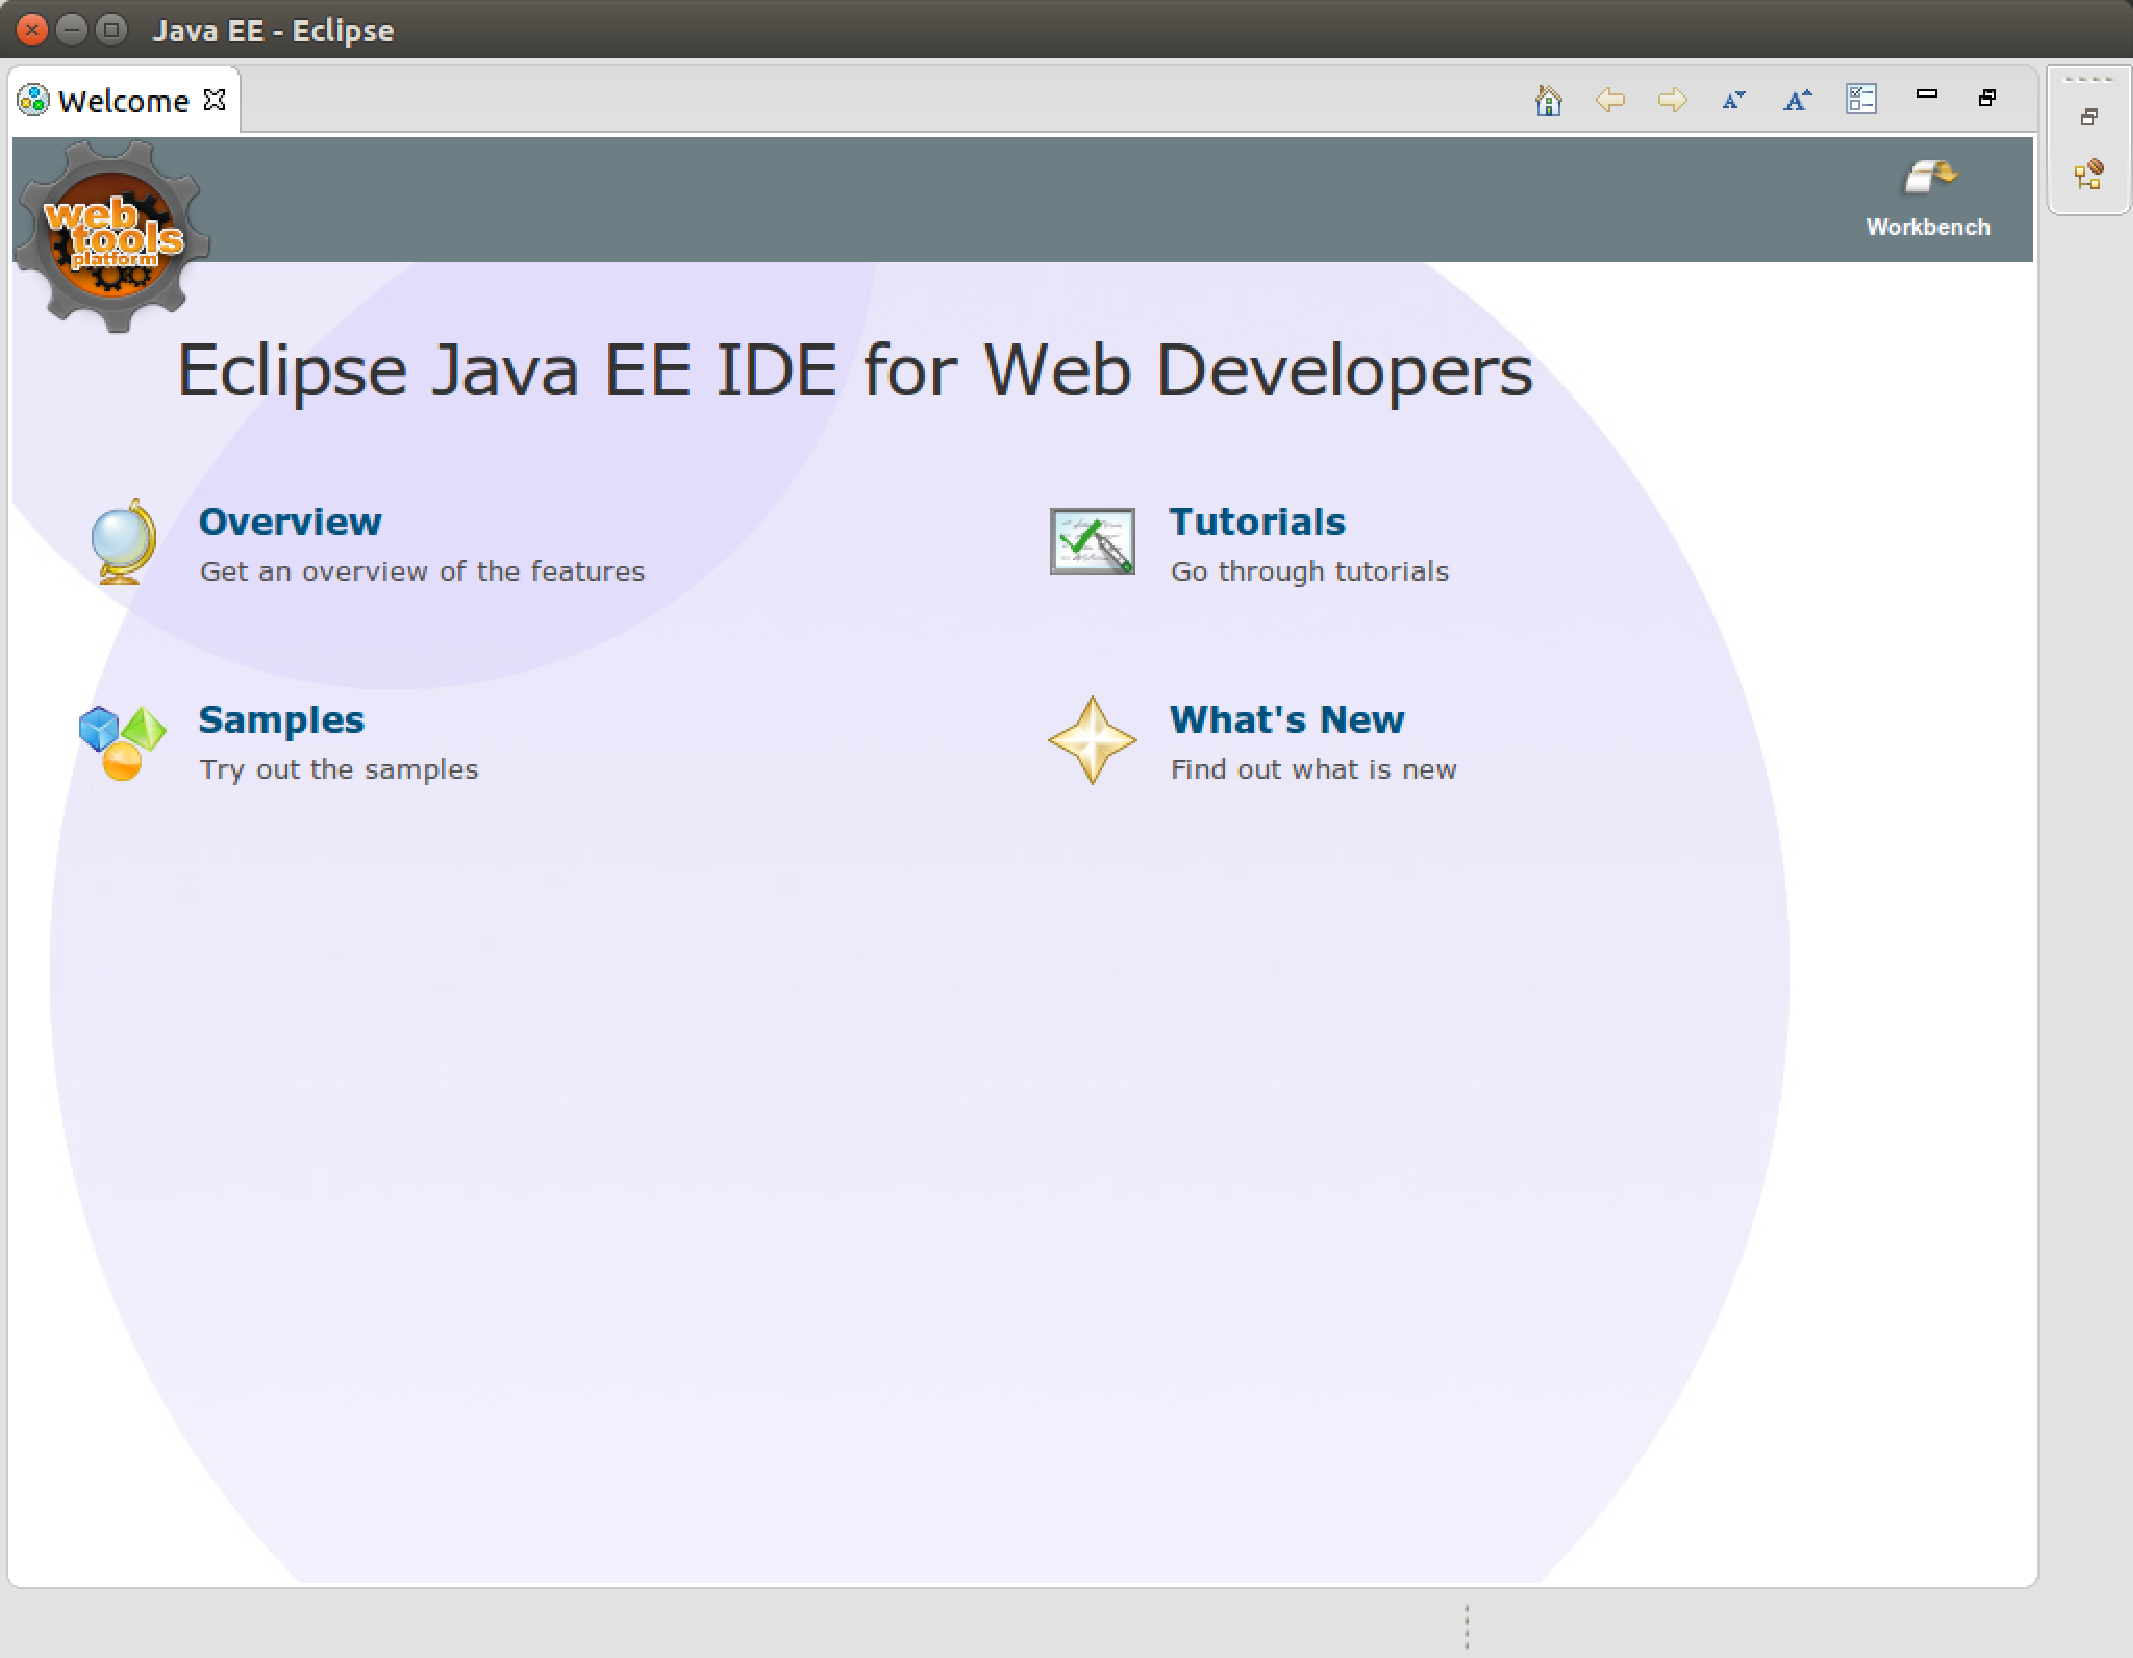
\includepdf[pages={1}]{img/eclipse/welcome.pdf}
}

% \pgfdeclareimage[height=\paperheight,width=\paperwidth]{start}{img/eclipse/start.png}
% \begin{frame}{Avvio di Eclipse}
%   \begin{center}
%     \pgfuseimage{start}
%   \end{center}
% \end{frame}
{
  \setbeamercolor{background canvas}{bg=}
  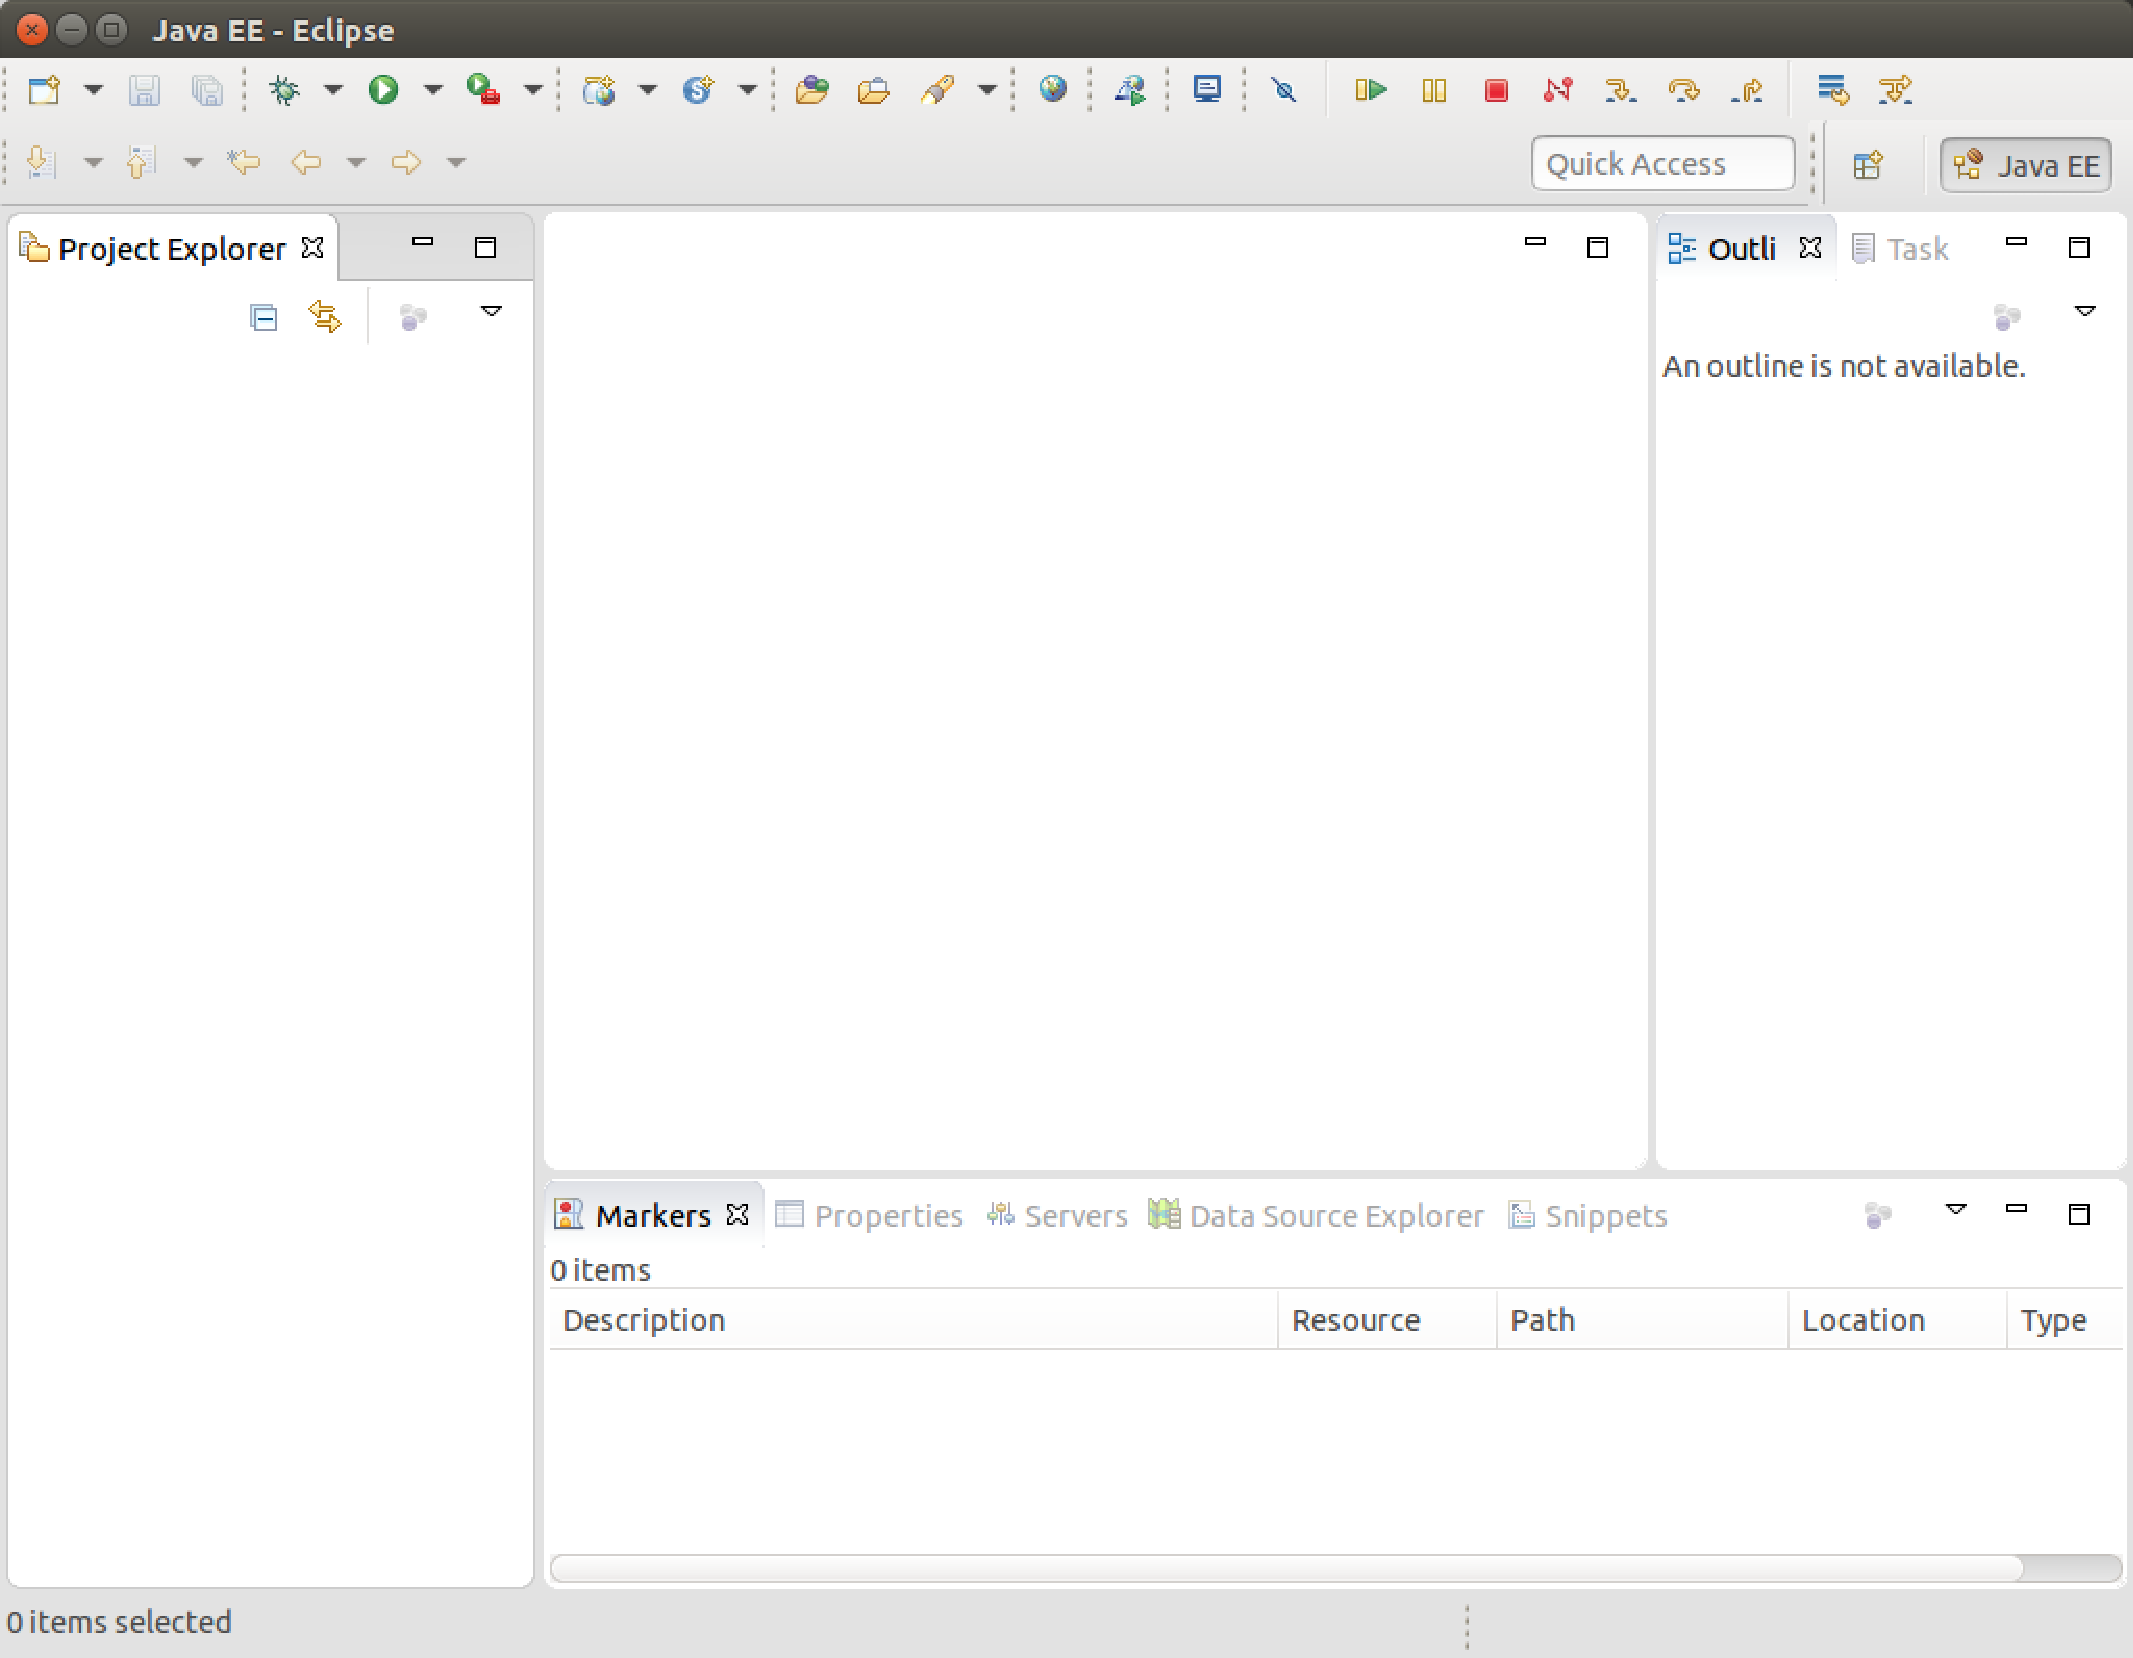
\includepdf[pages={1}]{img/eclipse/start.pdf}
}

% \pgfdeclareimage[height=\paperheight,width=\paperwidth]{new_project}{img/eclipse/new_project.png}
% \begin{frame}{Avvio di Eclipse}
%   \begin{center}
%     \pgfuseimage{new_project}
%   \end{center}
% \end{frame}
{
  \setbeamercolor{background canvas}{bg=}
  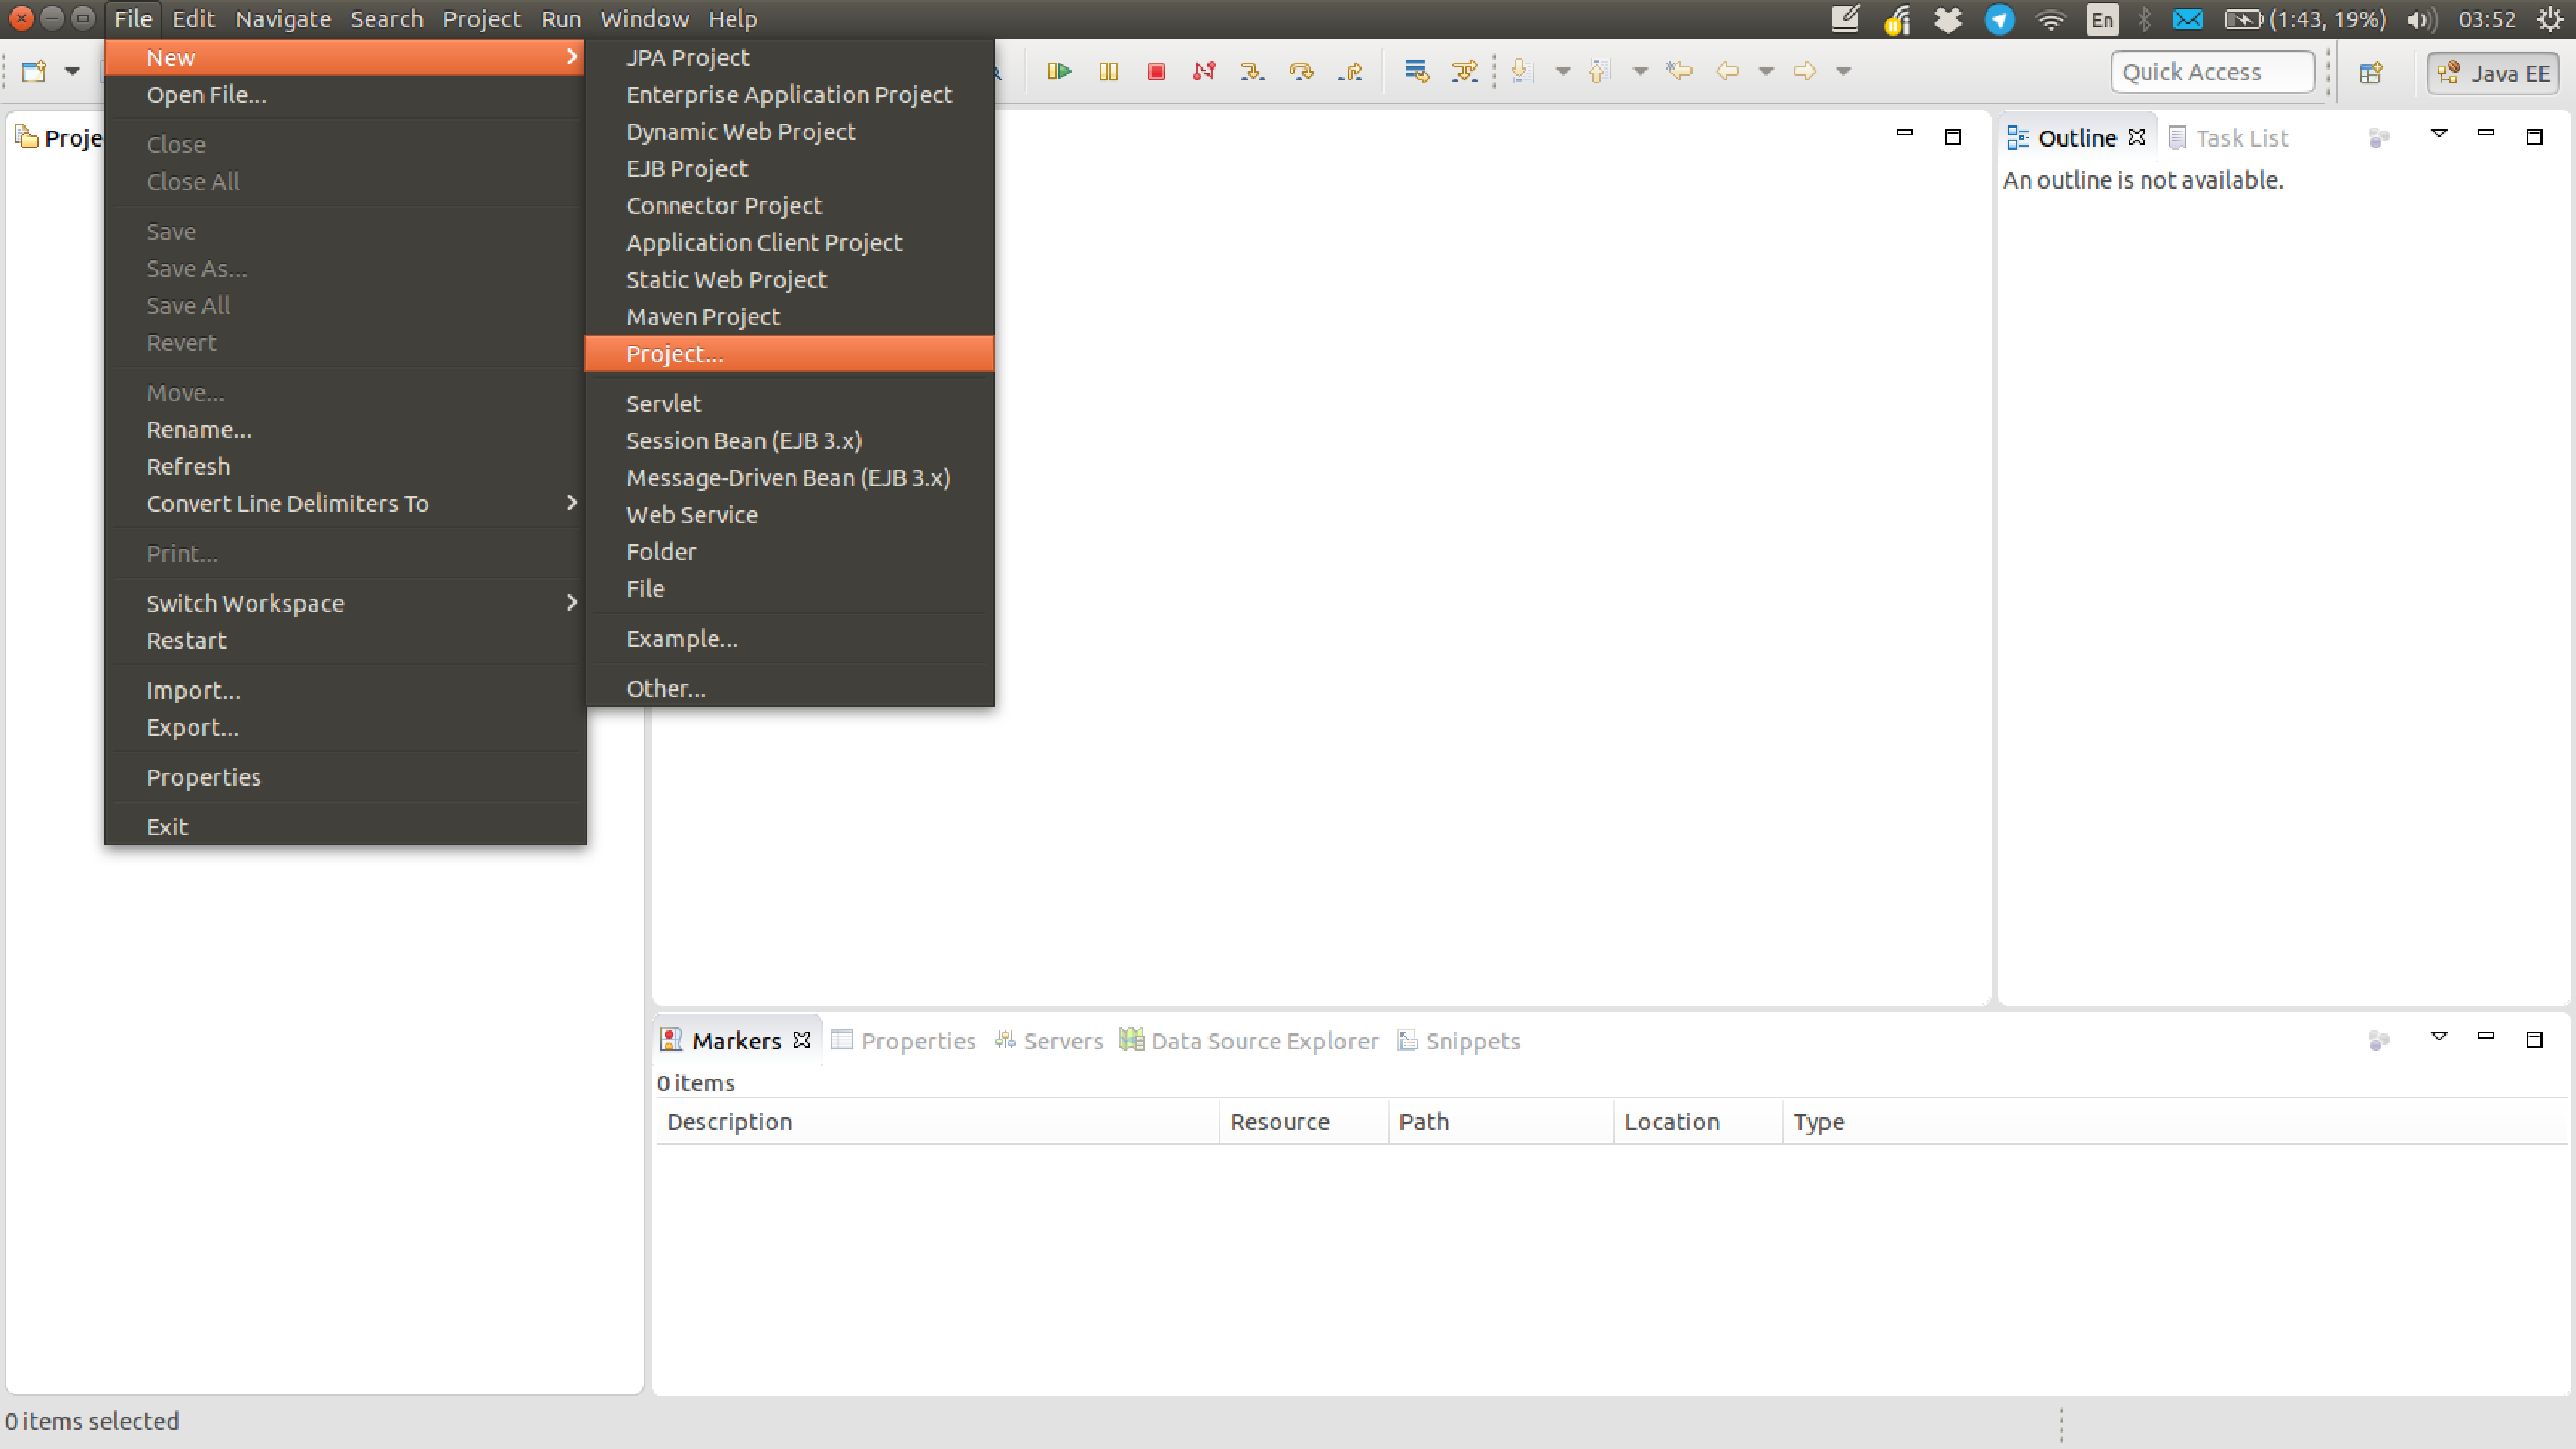
\includepdf[pages={1}]{img/eclipse/new_project.pdf}
}

% \pgfdeclareimage[height=\paperheight,width=\paperwidth]{new_java_project}{img/eclipse/new_java_project.png}
% \begin{frame}{Avvio di Eclipse}
%   \begin{center}
%     \pgfuseimage{new_java_project}
%   \end{center}
% \end{frame}
{
  \setbeamercolor{background canvas}{bg=}
  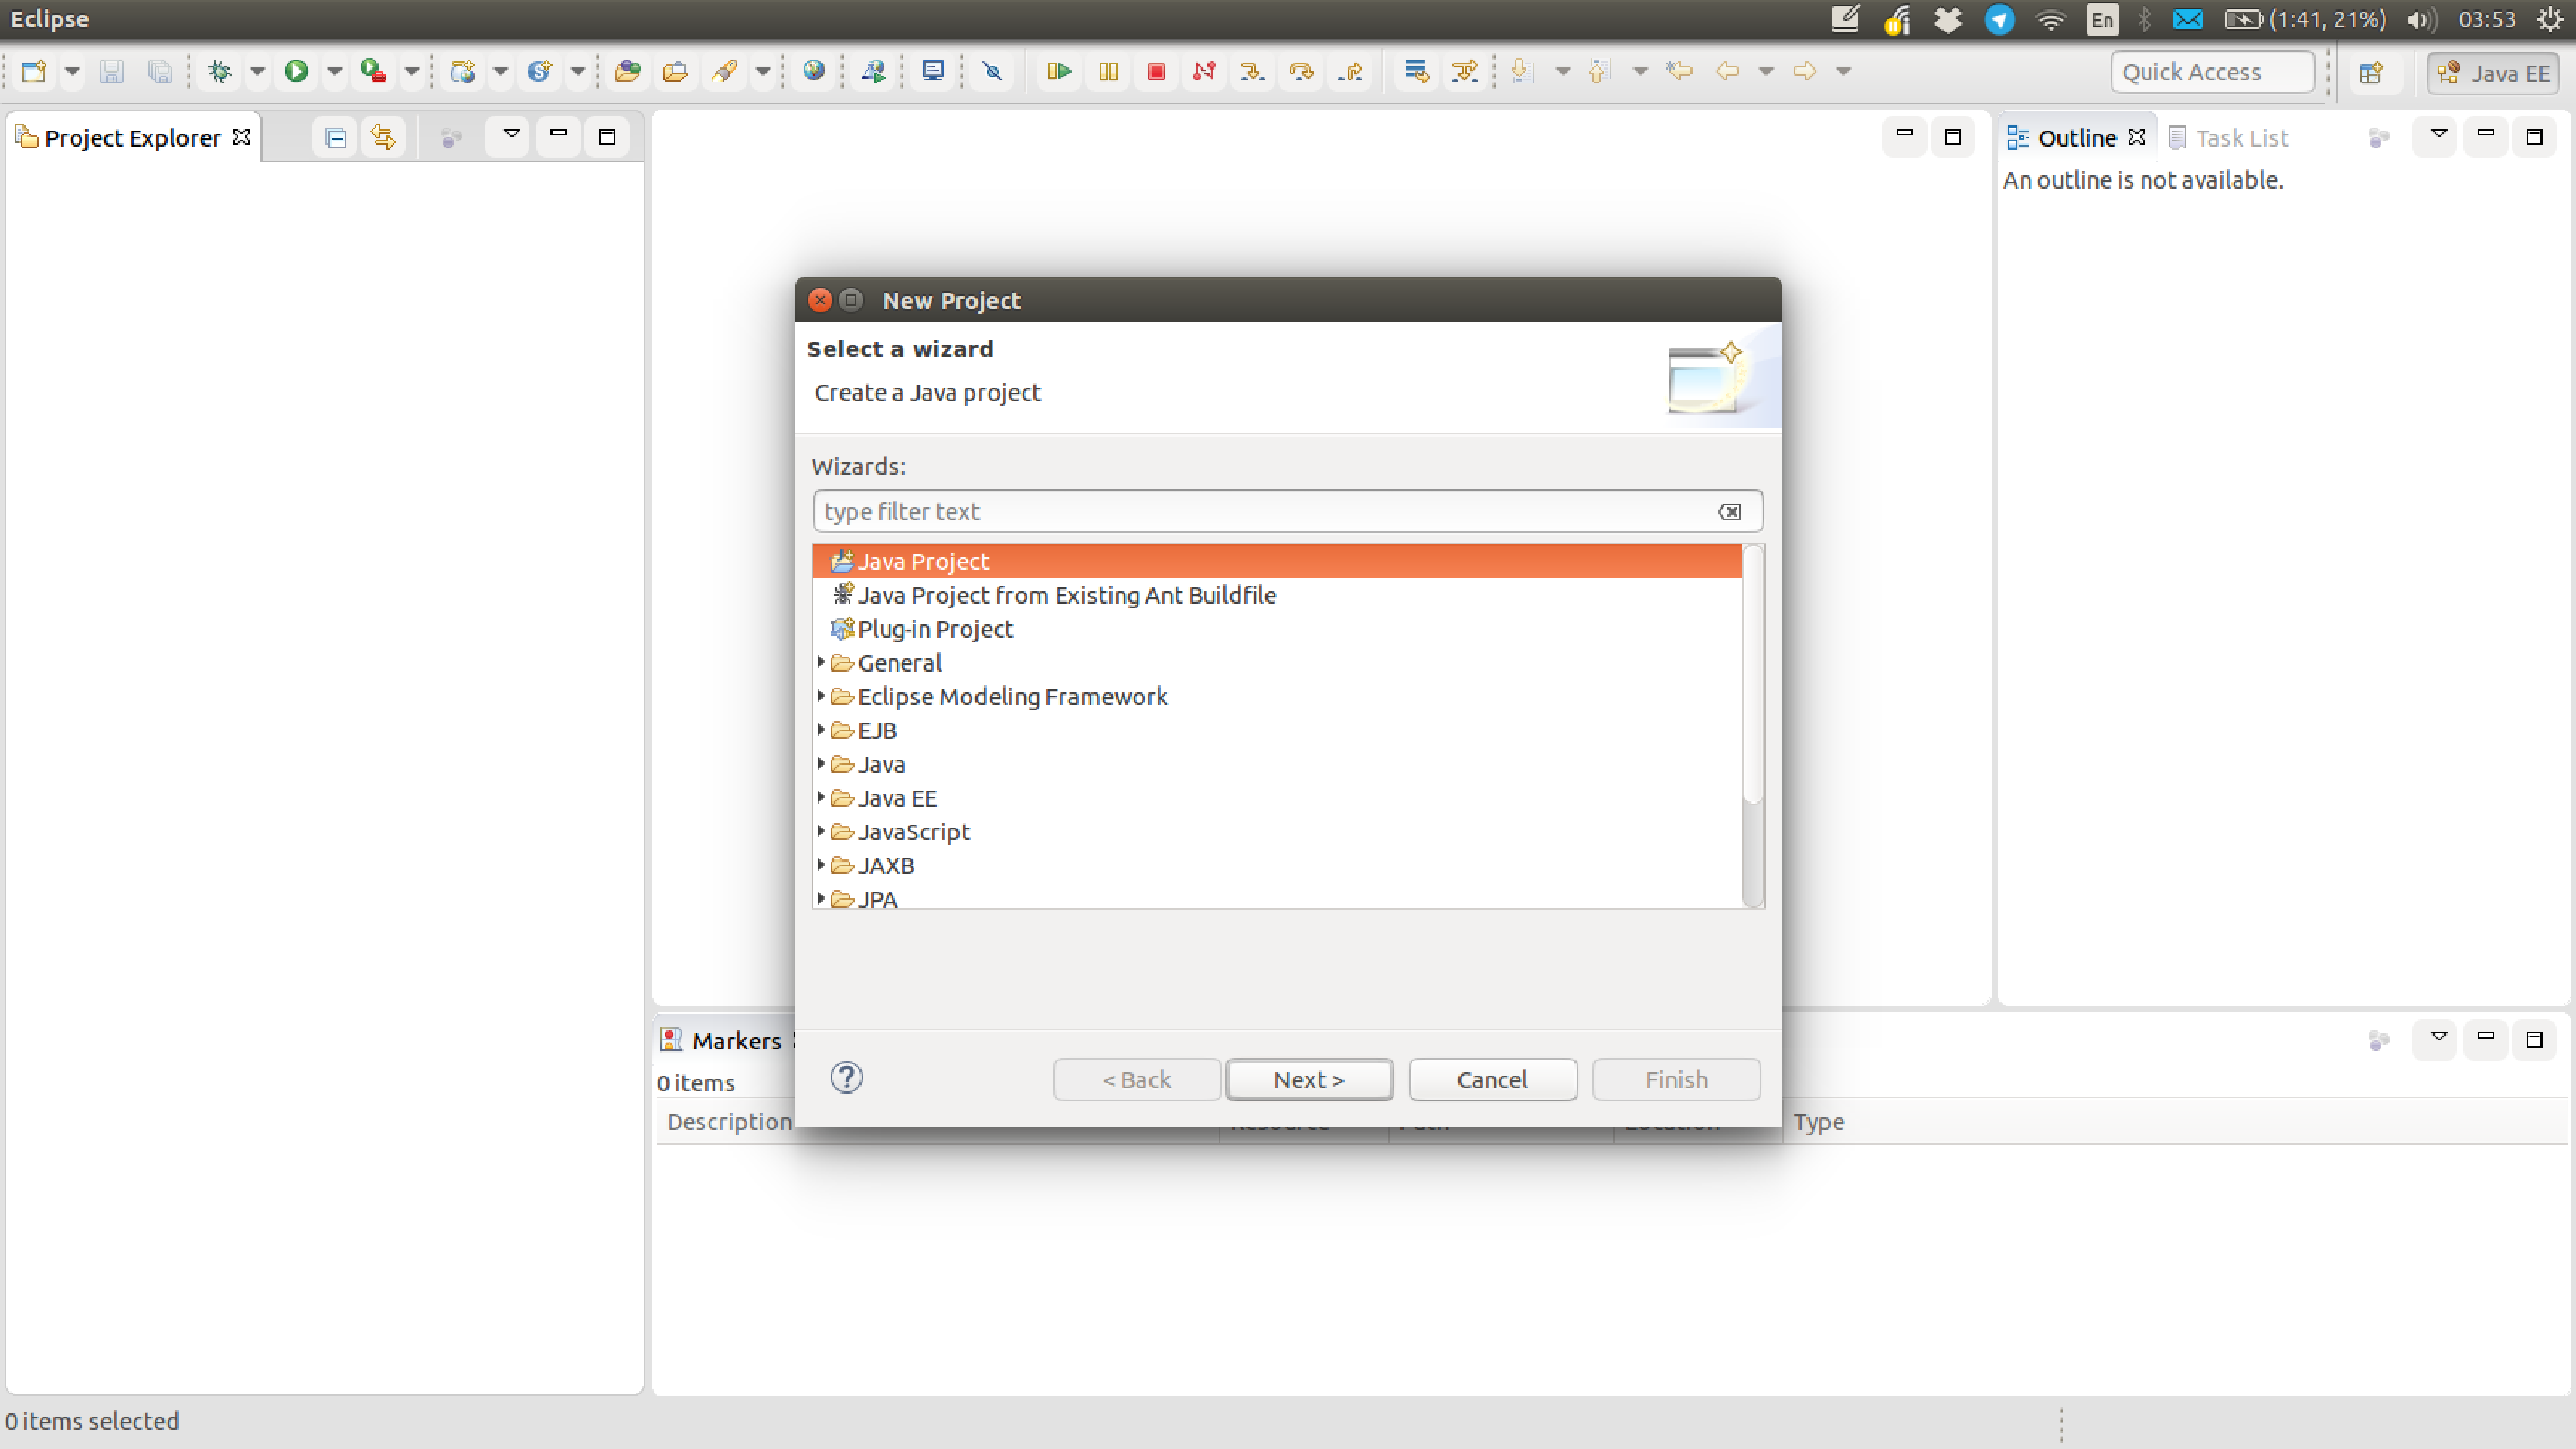
\includepdf[pages={1}]{img/eclipse/new_java_project.pdf}
}

% \pgfdeclareimage[height=\paperheight,width=\paperwidth]{create_project}{img/eclipse/create_project.png}
% \begin{frame}{Avvio di Eclipse}
%   \begin{center}
%     \pgfuseimage{create_project}
%   \end{center}
% \end{frame}
{
  \setbeamercolor{background canvas}{bg=}
  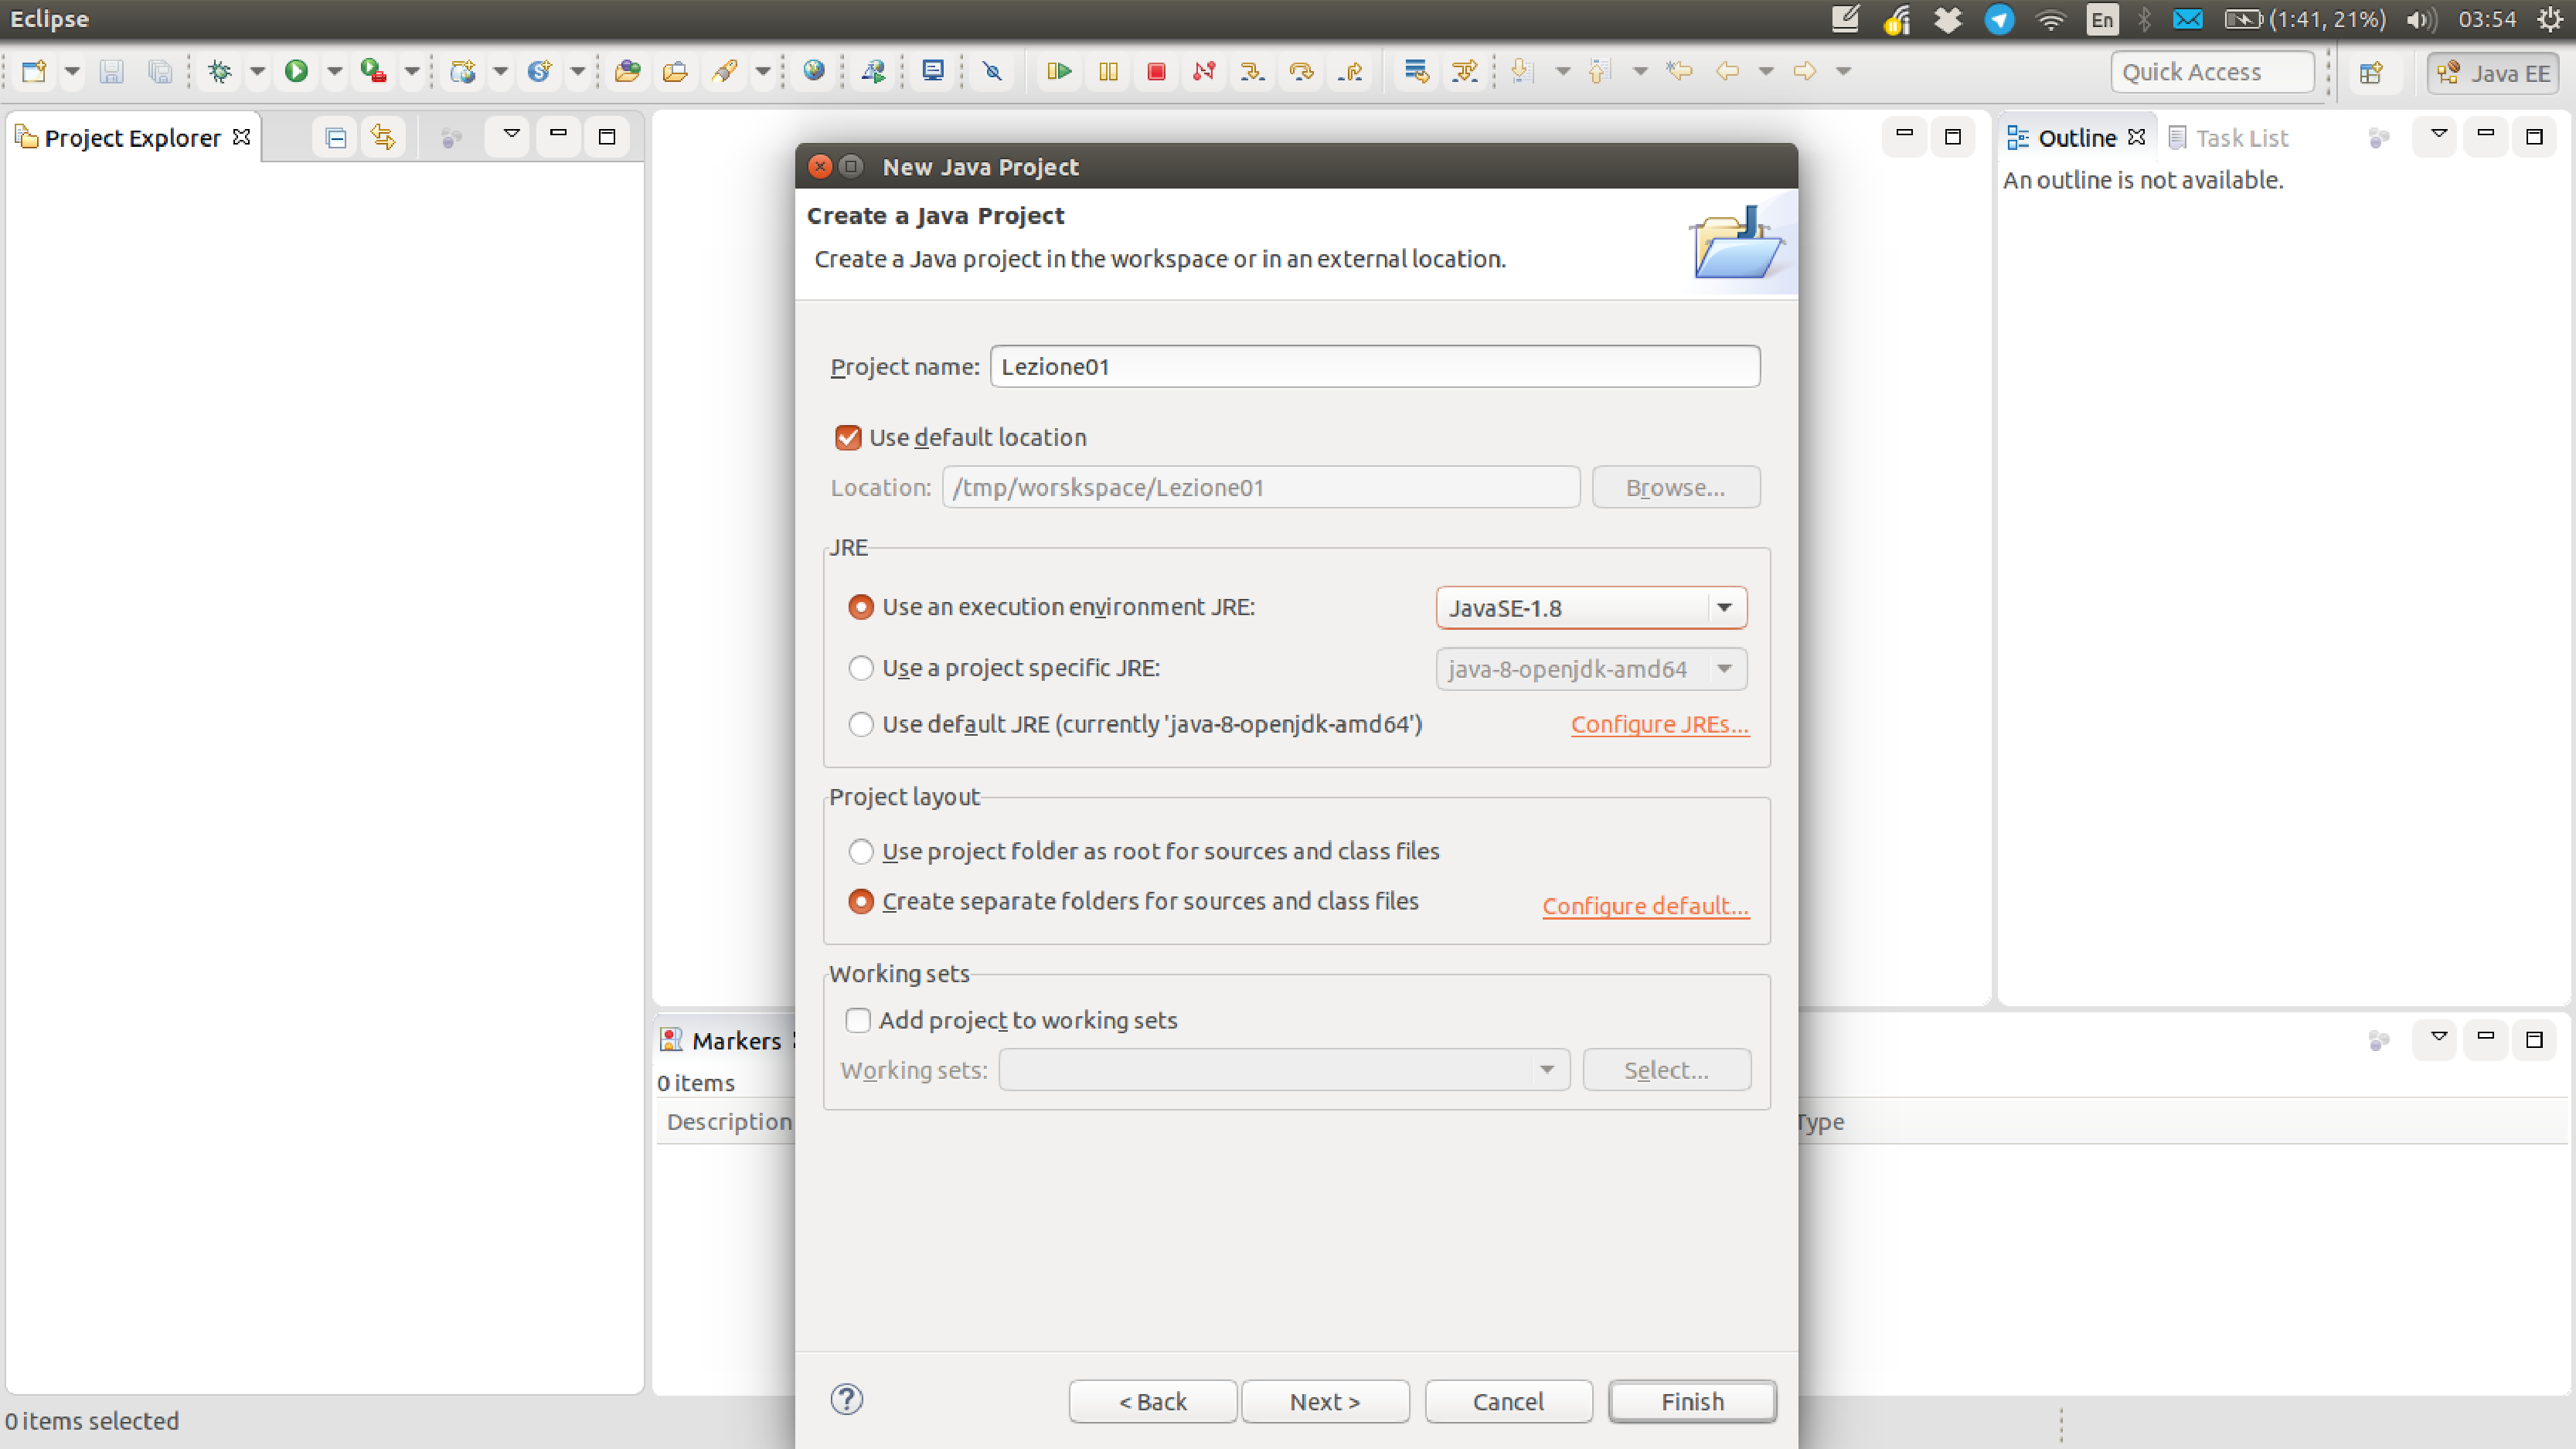
\includepdf[pages={1}]{img/eclipse/create_project.pdf}
}

% \pgfdeclareimage[height=\paperheight,width=\paperwidth]{project_created}{img/eclipse/project_created.png}
% \begin{frame}{Avvio di Eclipse}
%   \begin{center}
%     \pgfuseimage{project_created}
%   \end{center}
% \end{frame}
{
  \setbeamercolor{background canvas}{bg=}
  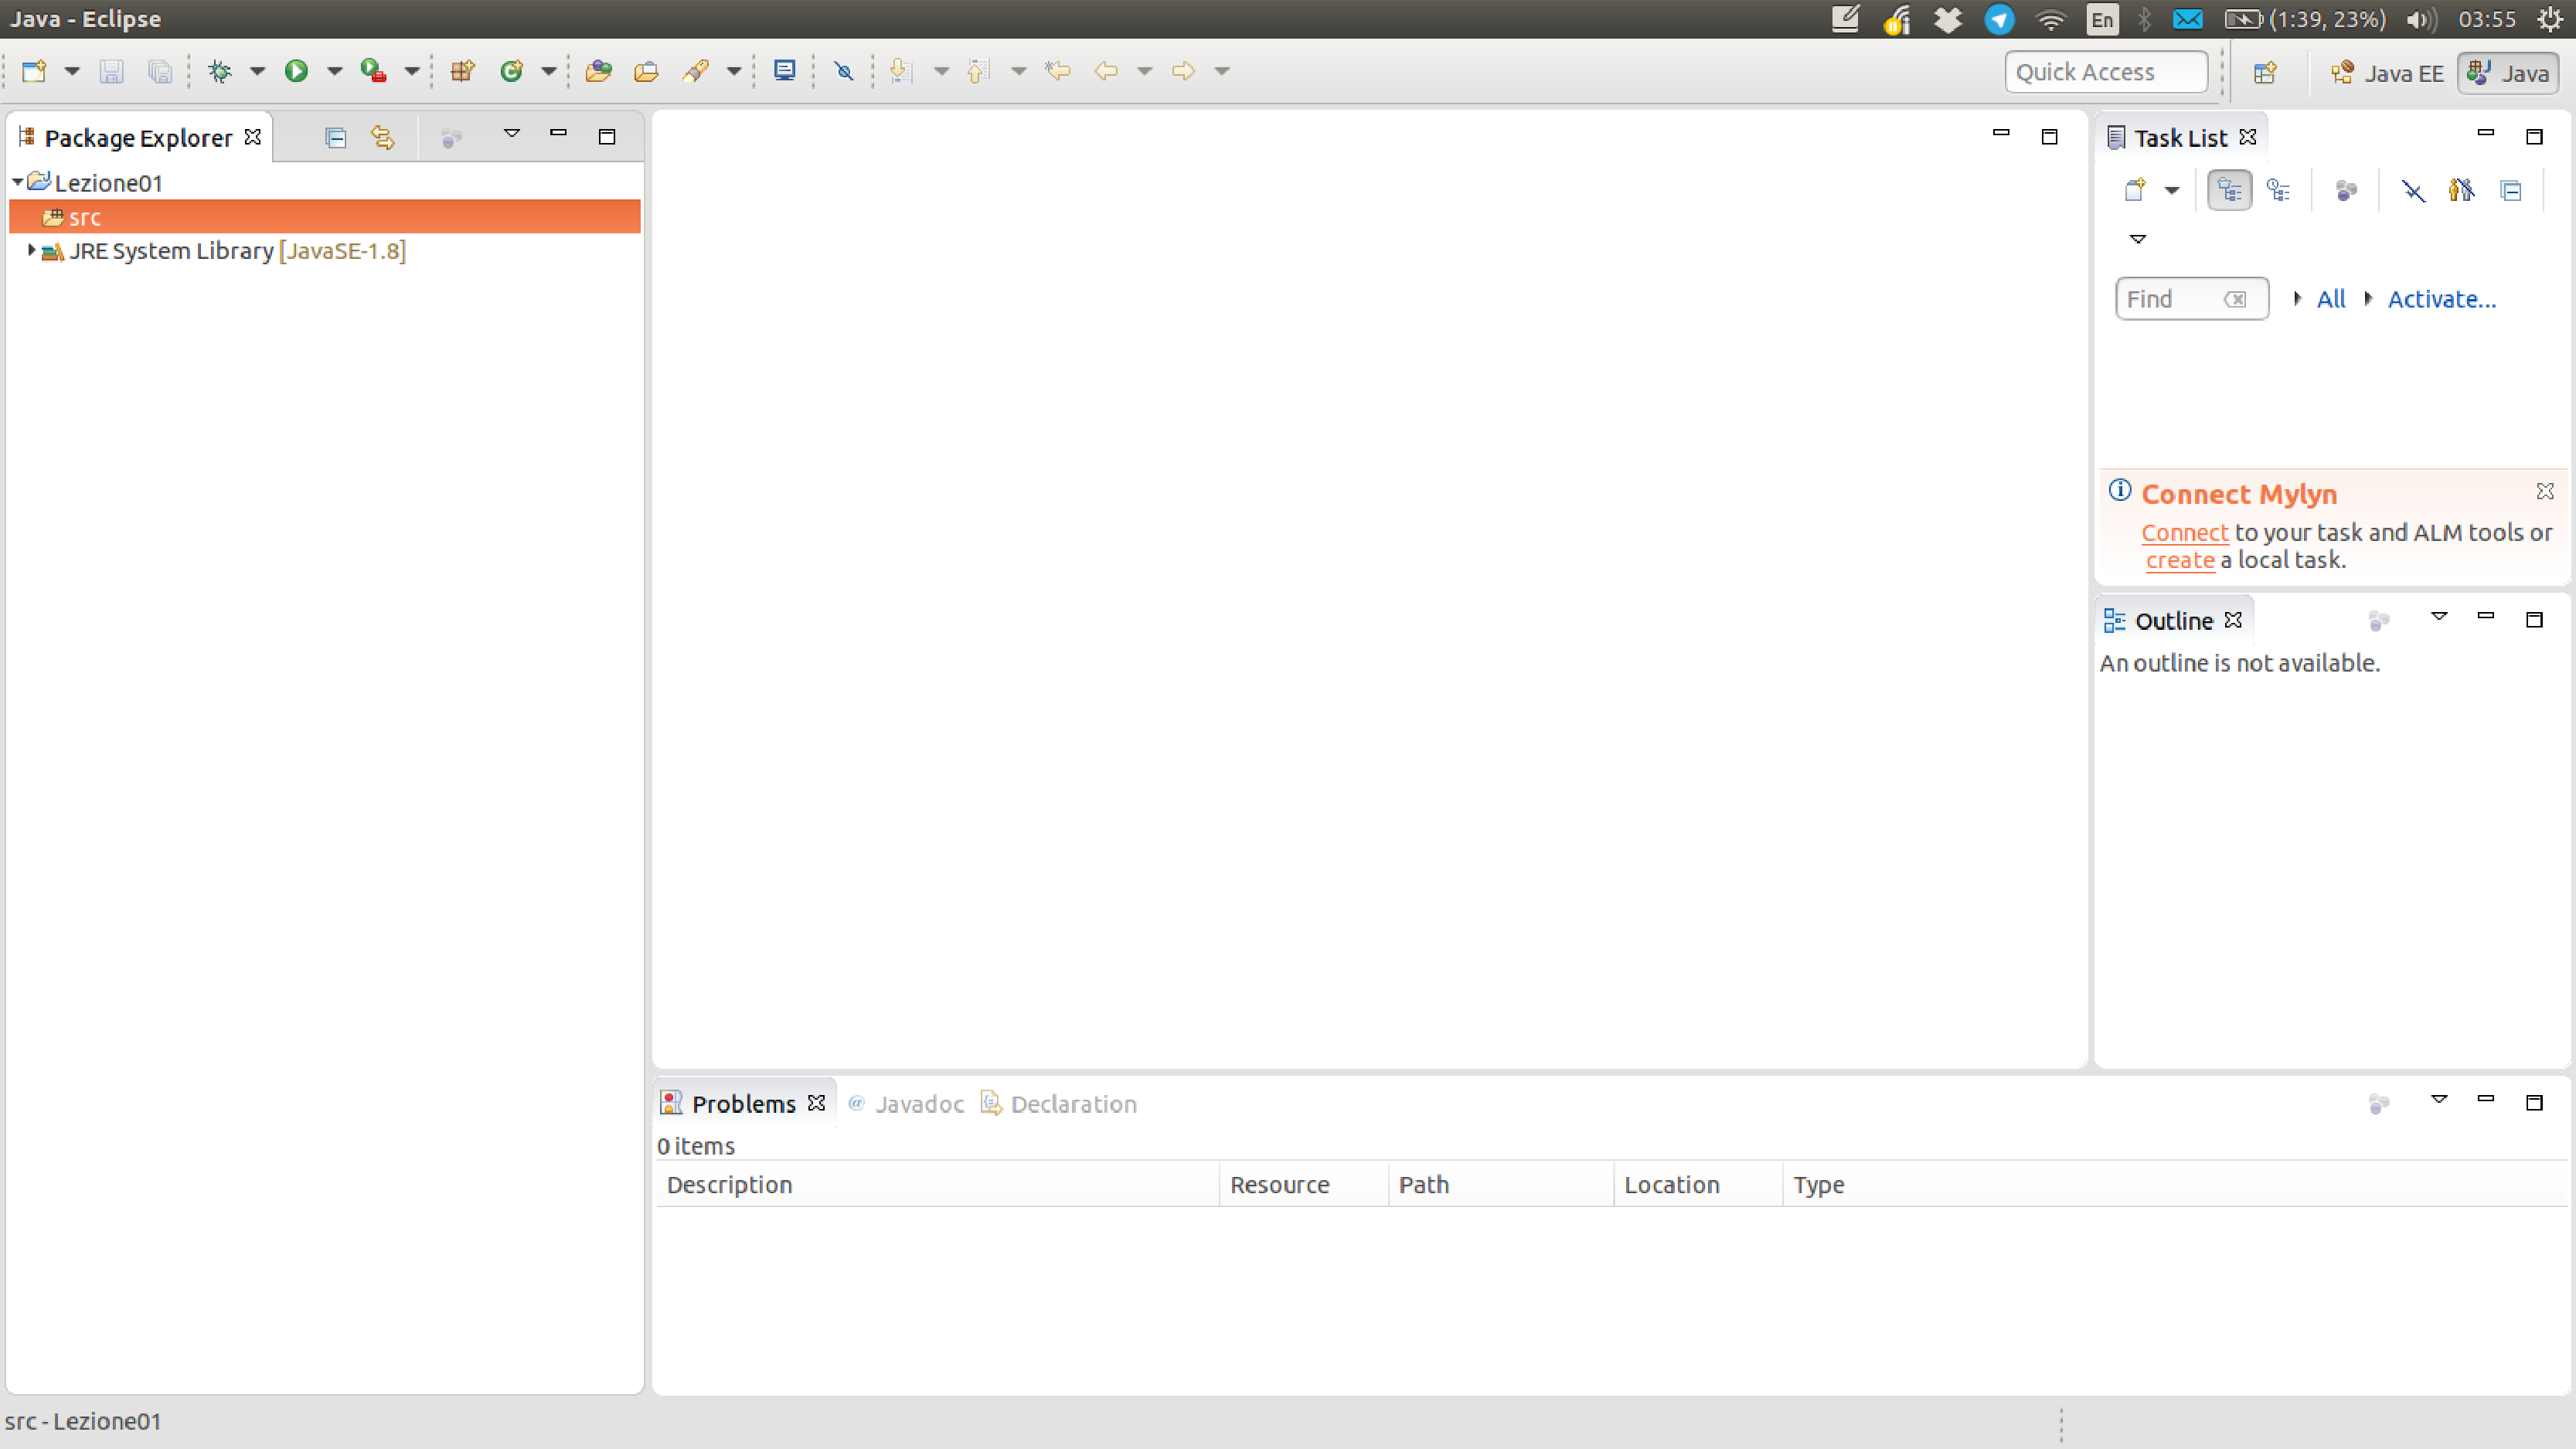
\includepdf[pages={1}]{img/eclipse/project_created.pdf}
}

% \pgfdeclareimage[height=\paperheight,width=\paperwidth]{new_class}{img/eclipse/new_class.png}
% \begin{frame}{Avvio di Eclipse}
%   \begin{center}
%     \pgfuseimage{new_class}
%   \end{center}
% \end{frame}
{
  \setbeamercolor{background canvas}{bg=}
  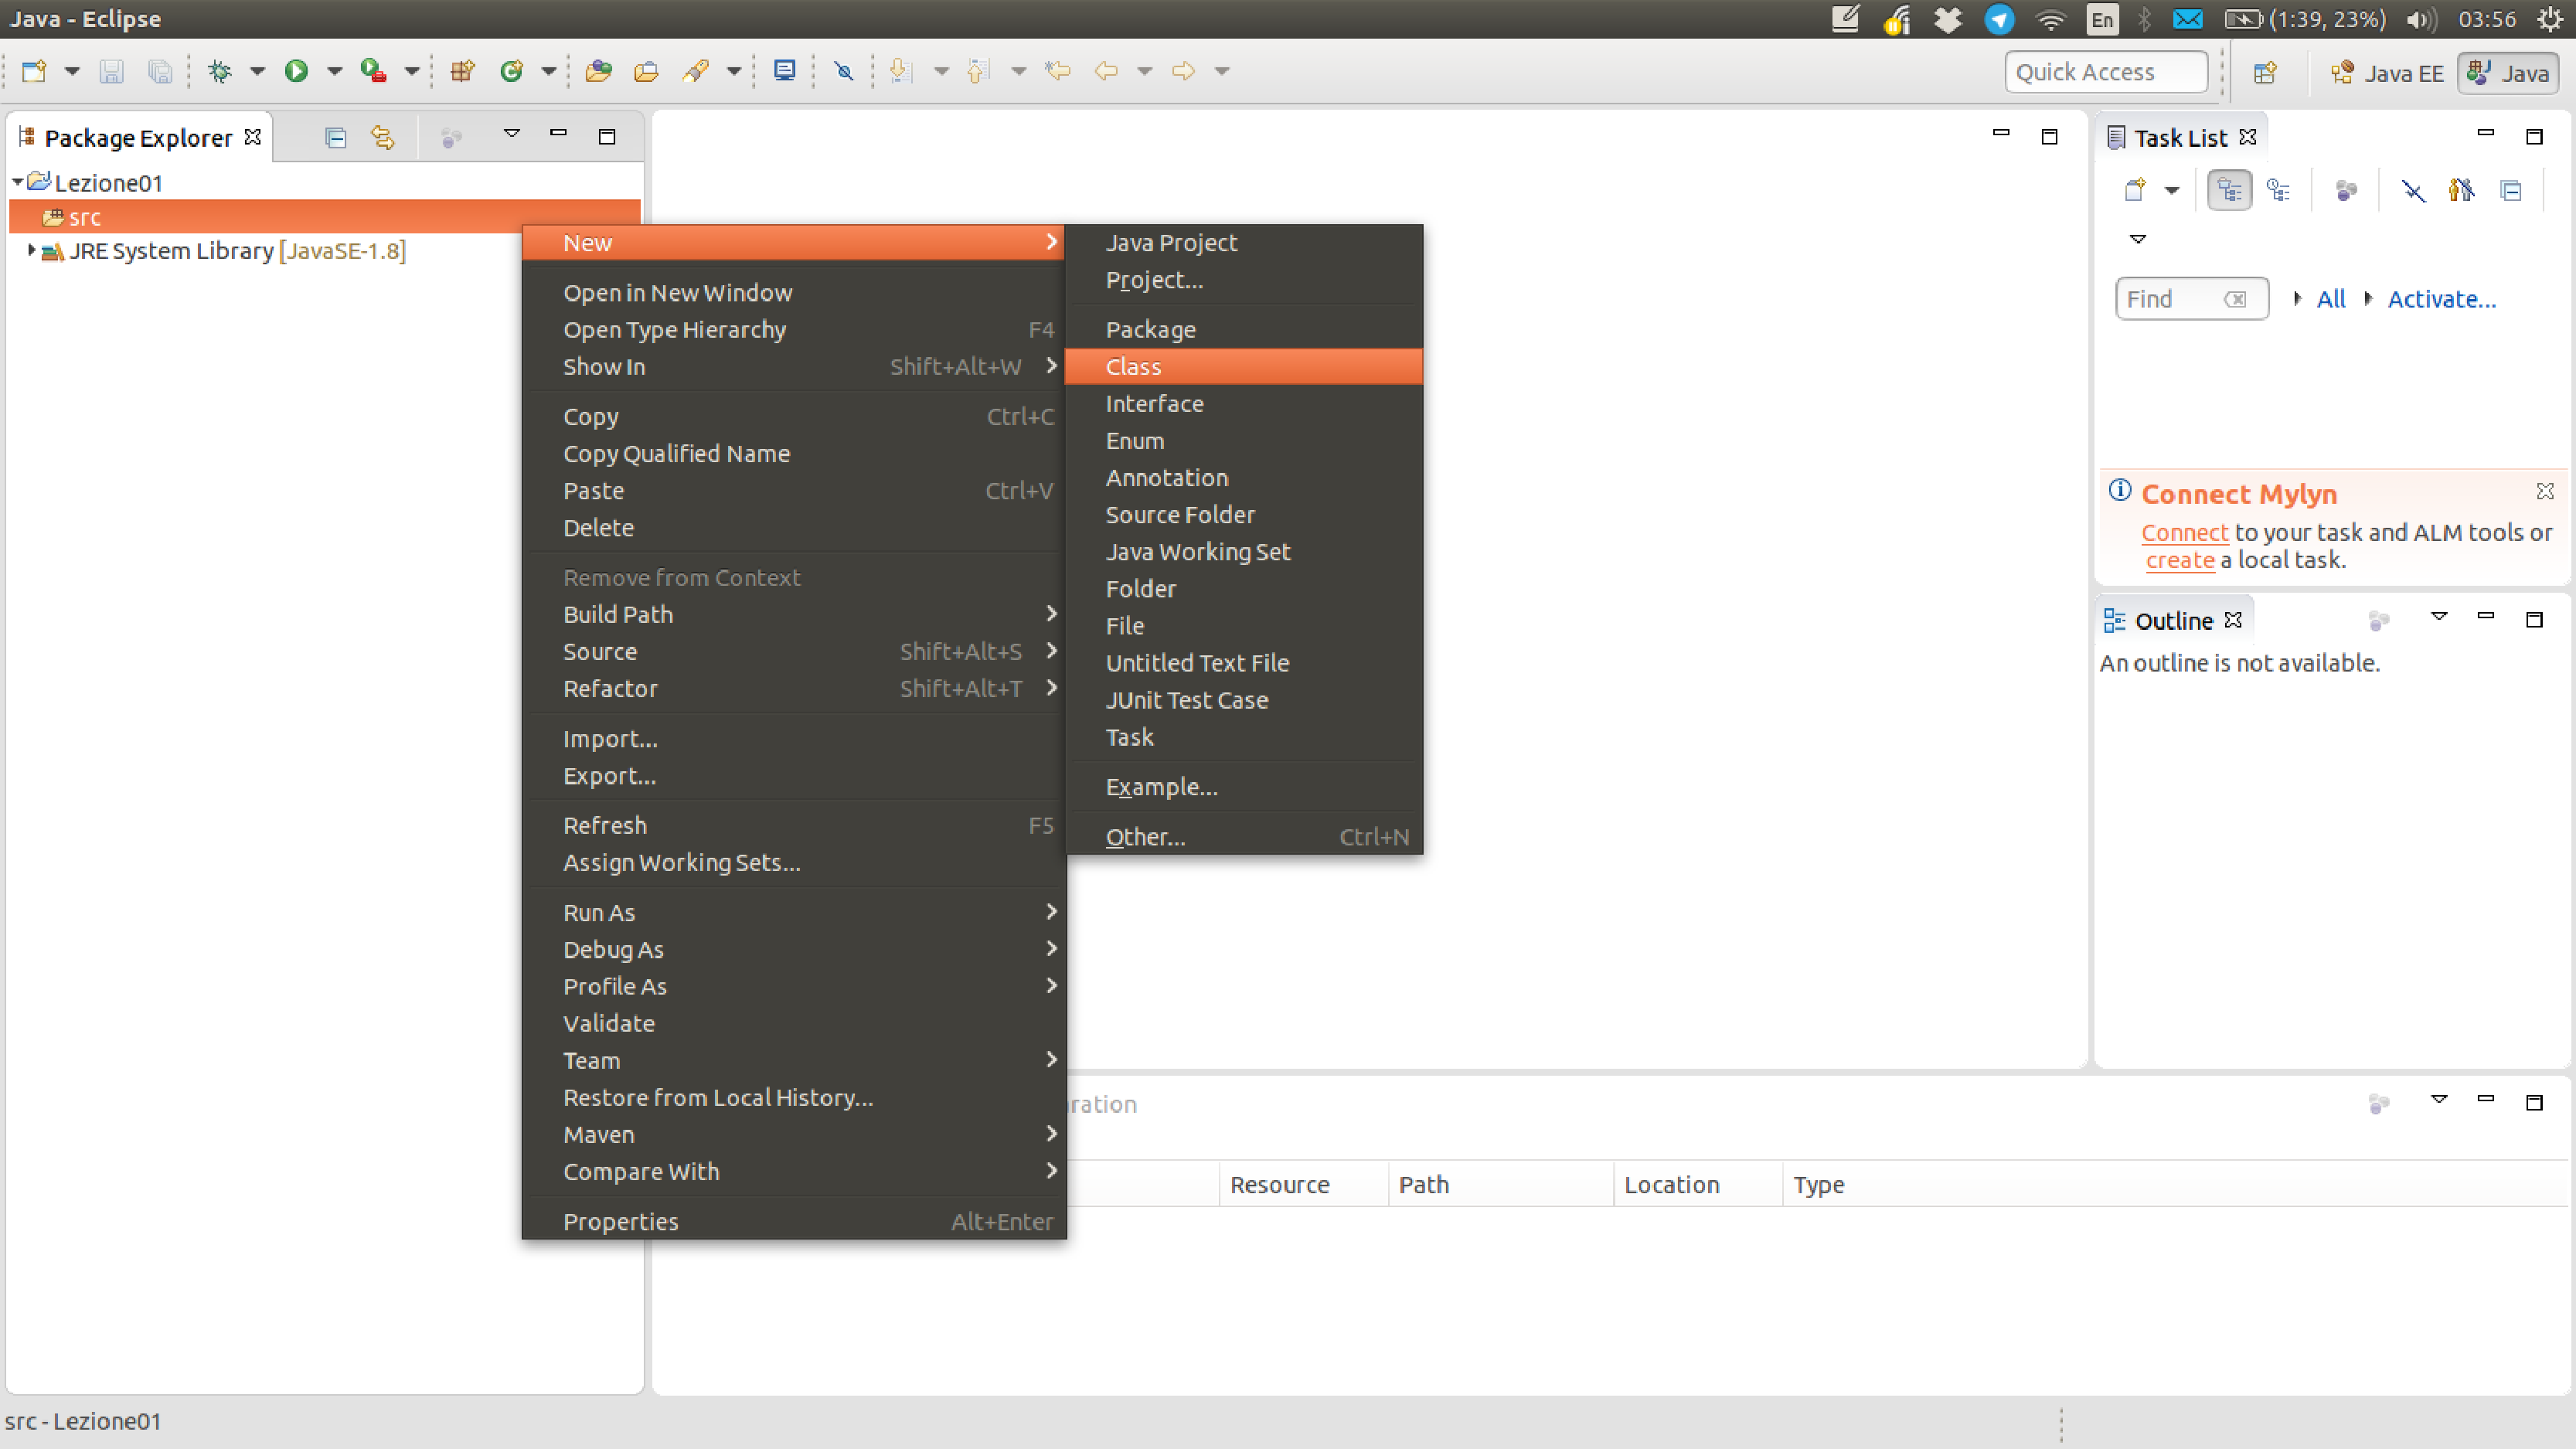
\includepdf[pages={1}]{img/eclipse/new_class.pdf}
}

% \pgfdeclareimage[height=\paperheight,width=\paperwidth]{create_class}{img/eclipse/create_class.png}
% \begin{frame}{Avvio di Eclipse}
%   \begin{center}
%     \pgfuseimage{create_class}
%   \end{center}
% \end{frame}
{
  \setbeamercolor{background canvas}{bg=}
  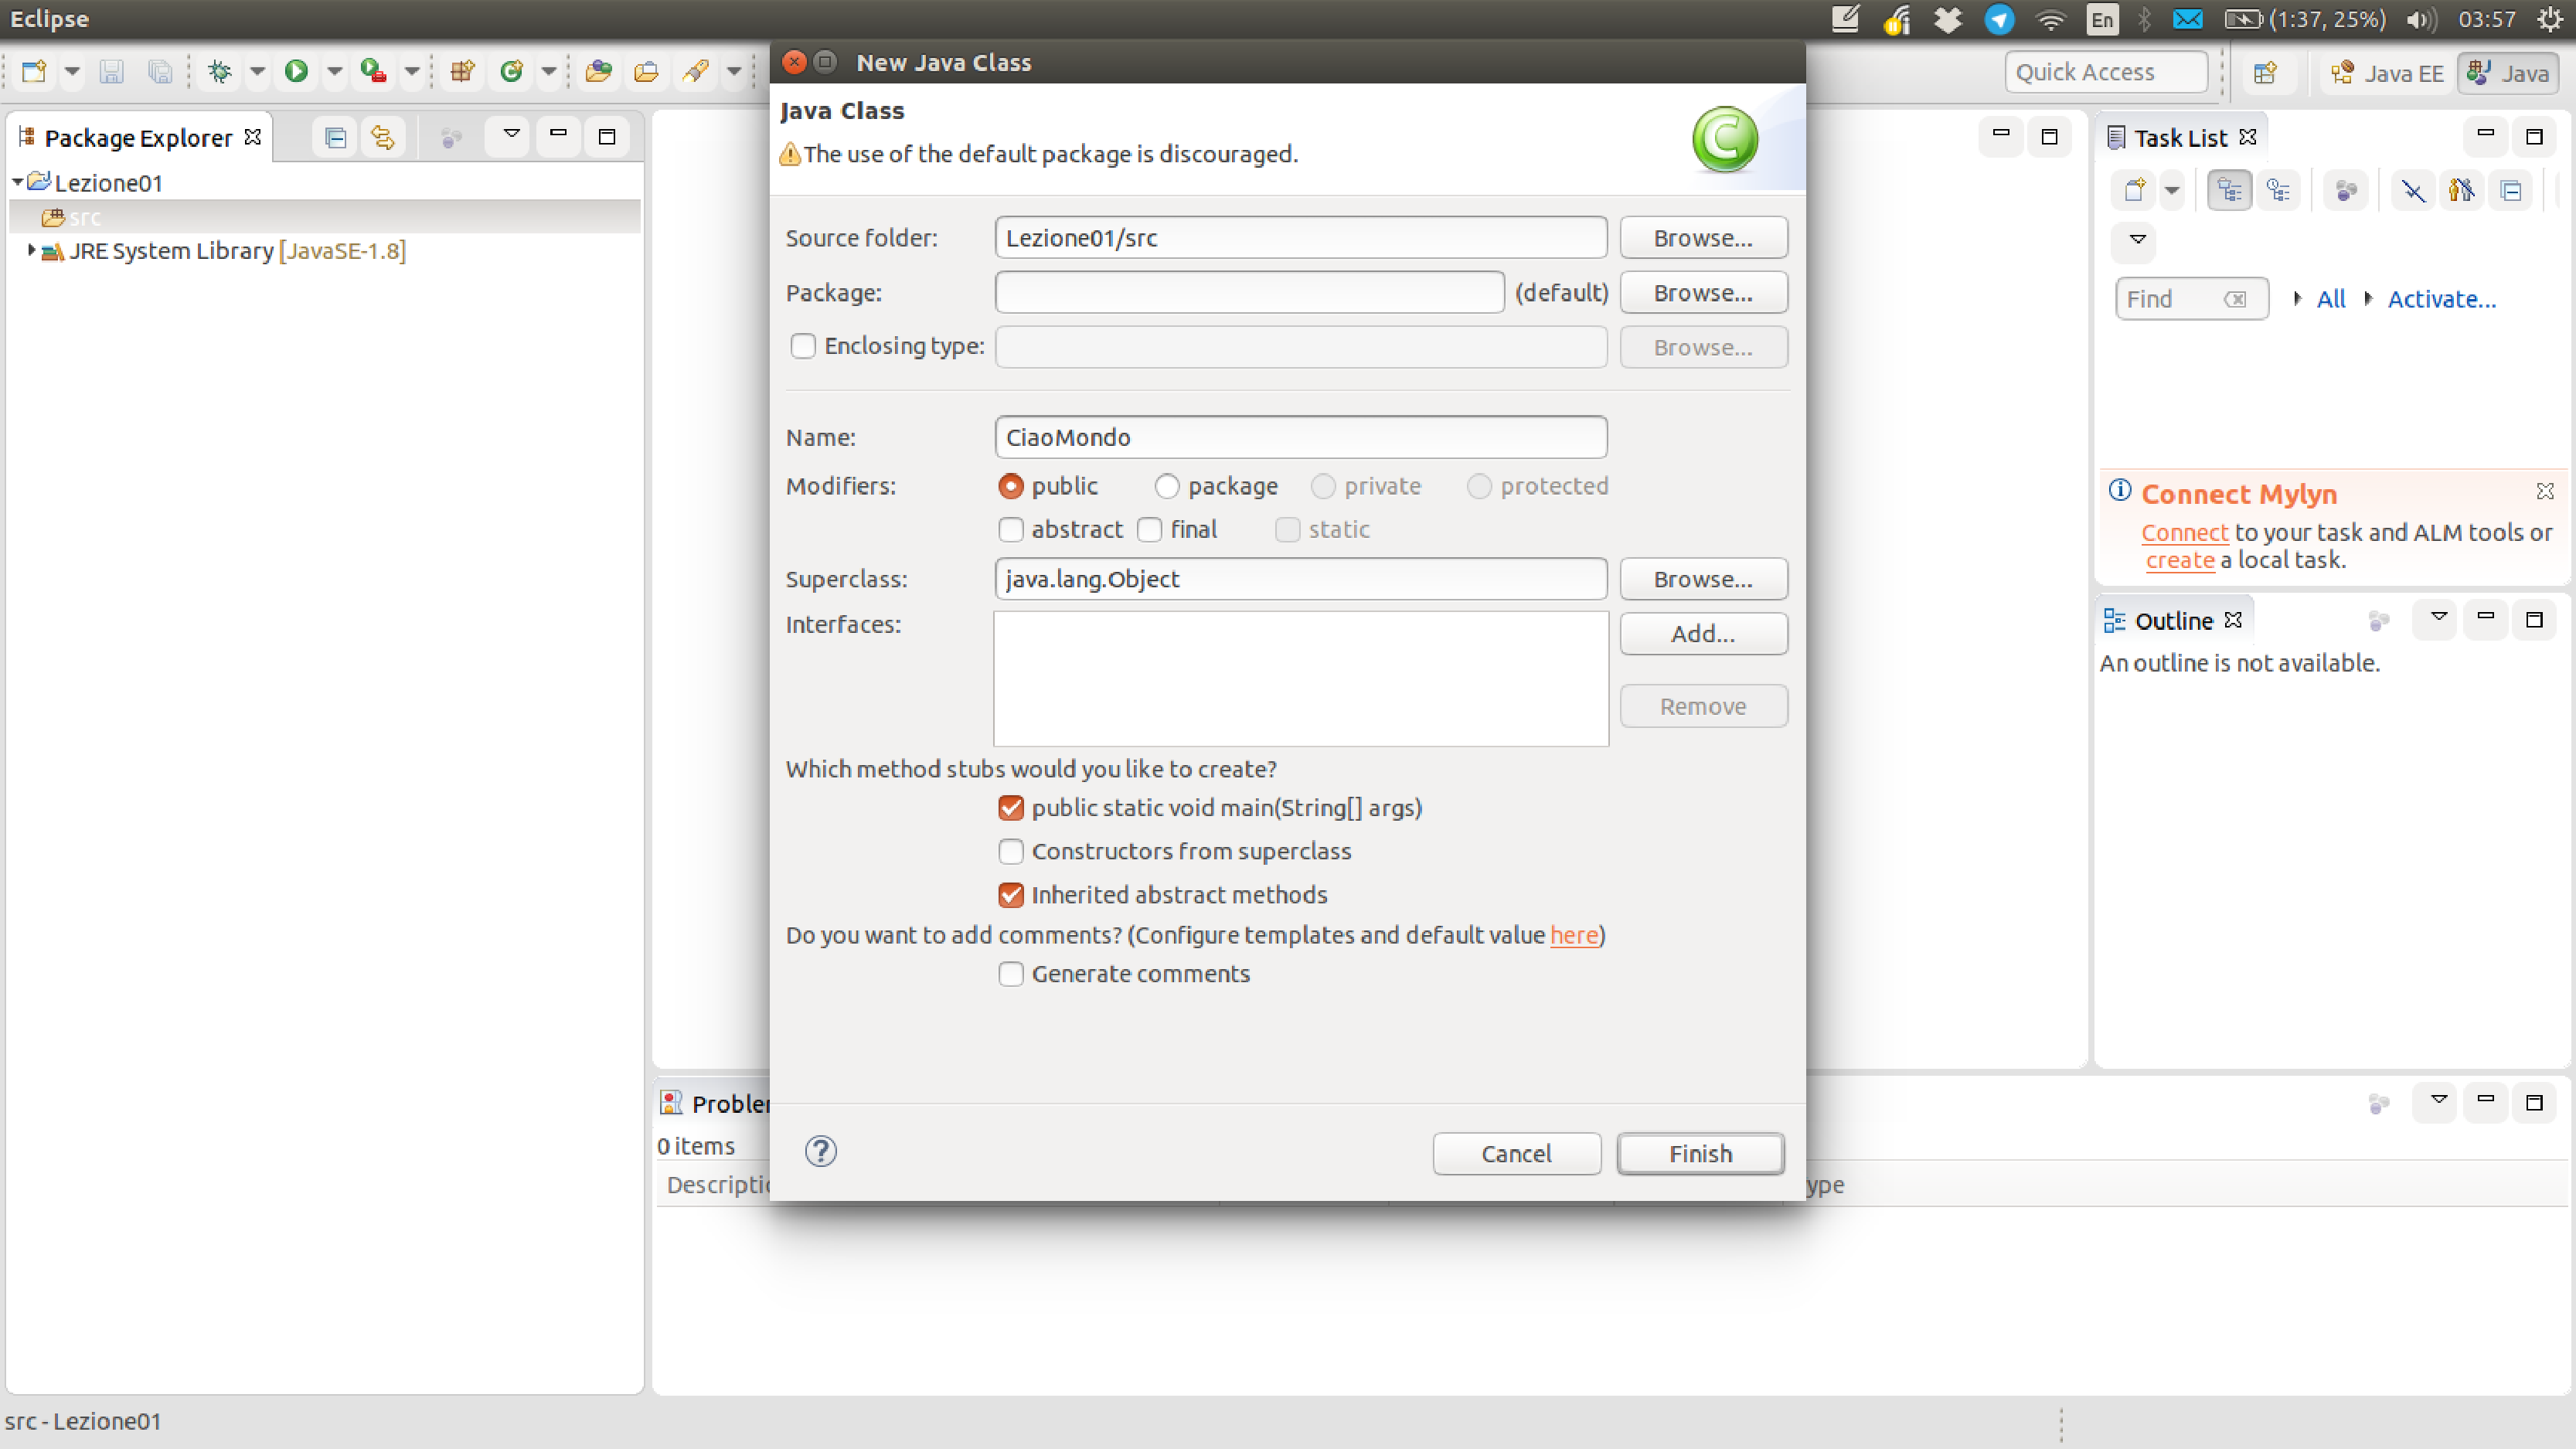
\includepdf[pages={1}]{img/eclipse/create_class.pdf}
}

% \pgfdeclareimage[height=\paperheight,width=\paperwidth]{class_created}{img/eclipse/class_created.png}
% \begin{frame}{Avvio di Eclipse}
%   \begin{center}
%     \pgfuseimage{class_created}
%   \end{center}
% \end{frame}
{
  \setbeamercolor{background canvas}{bg=}
  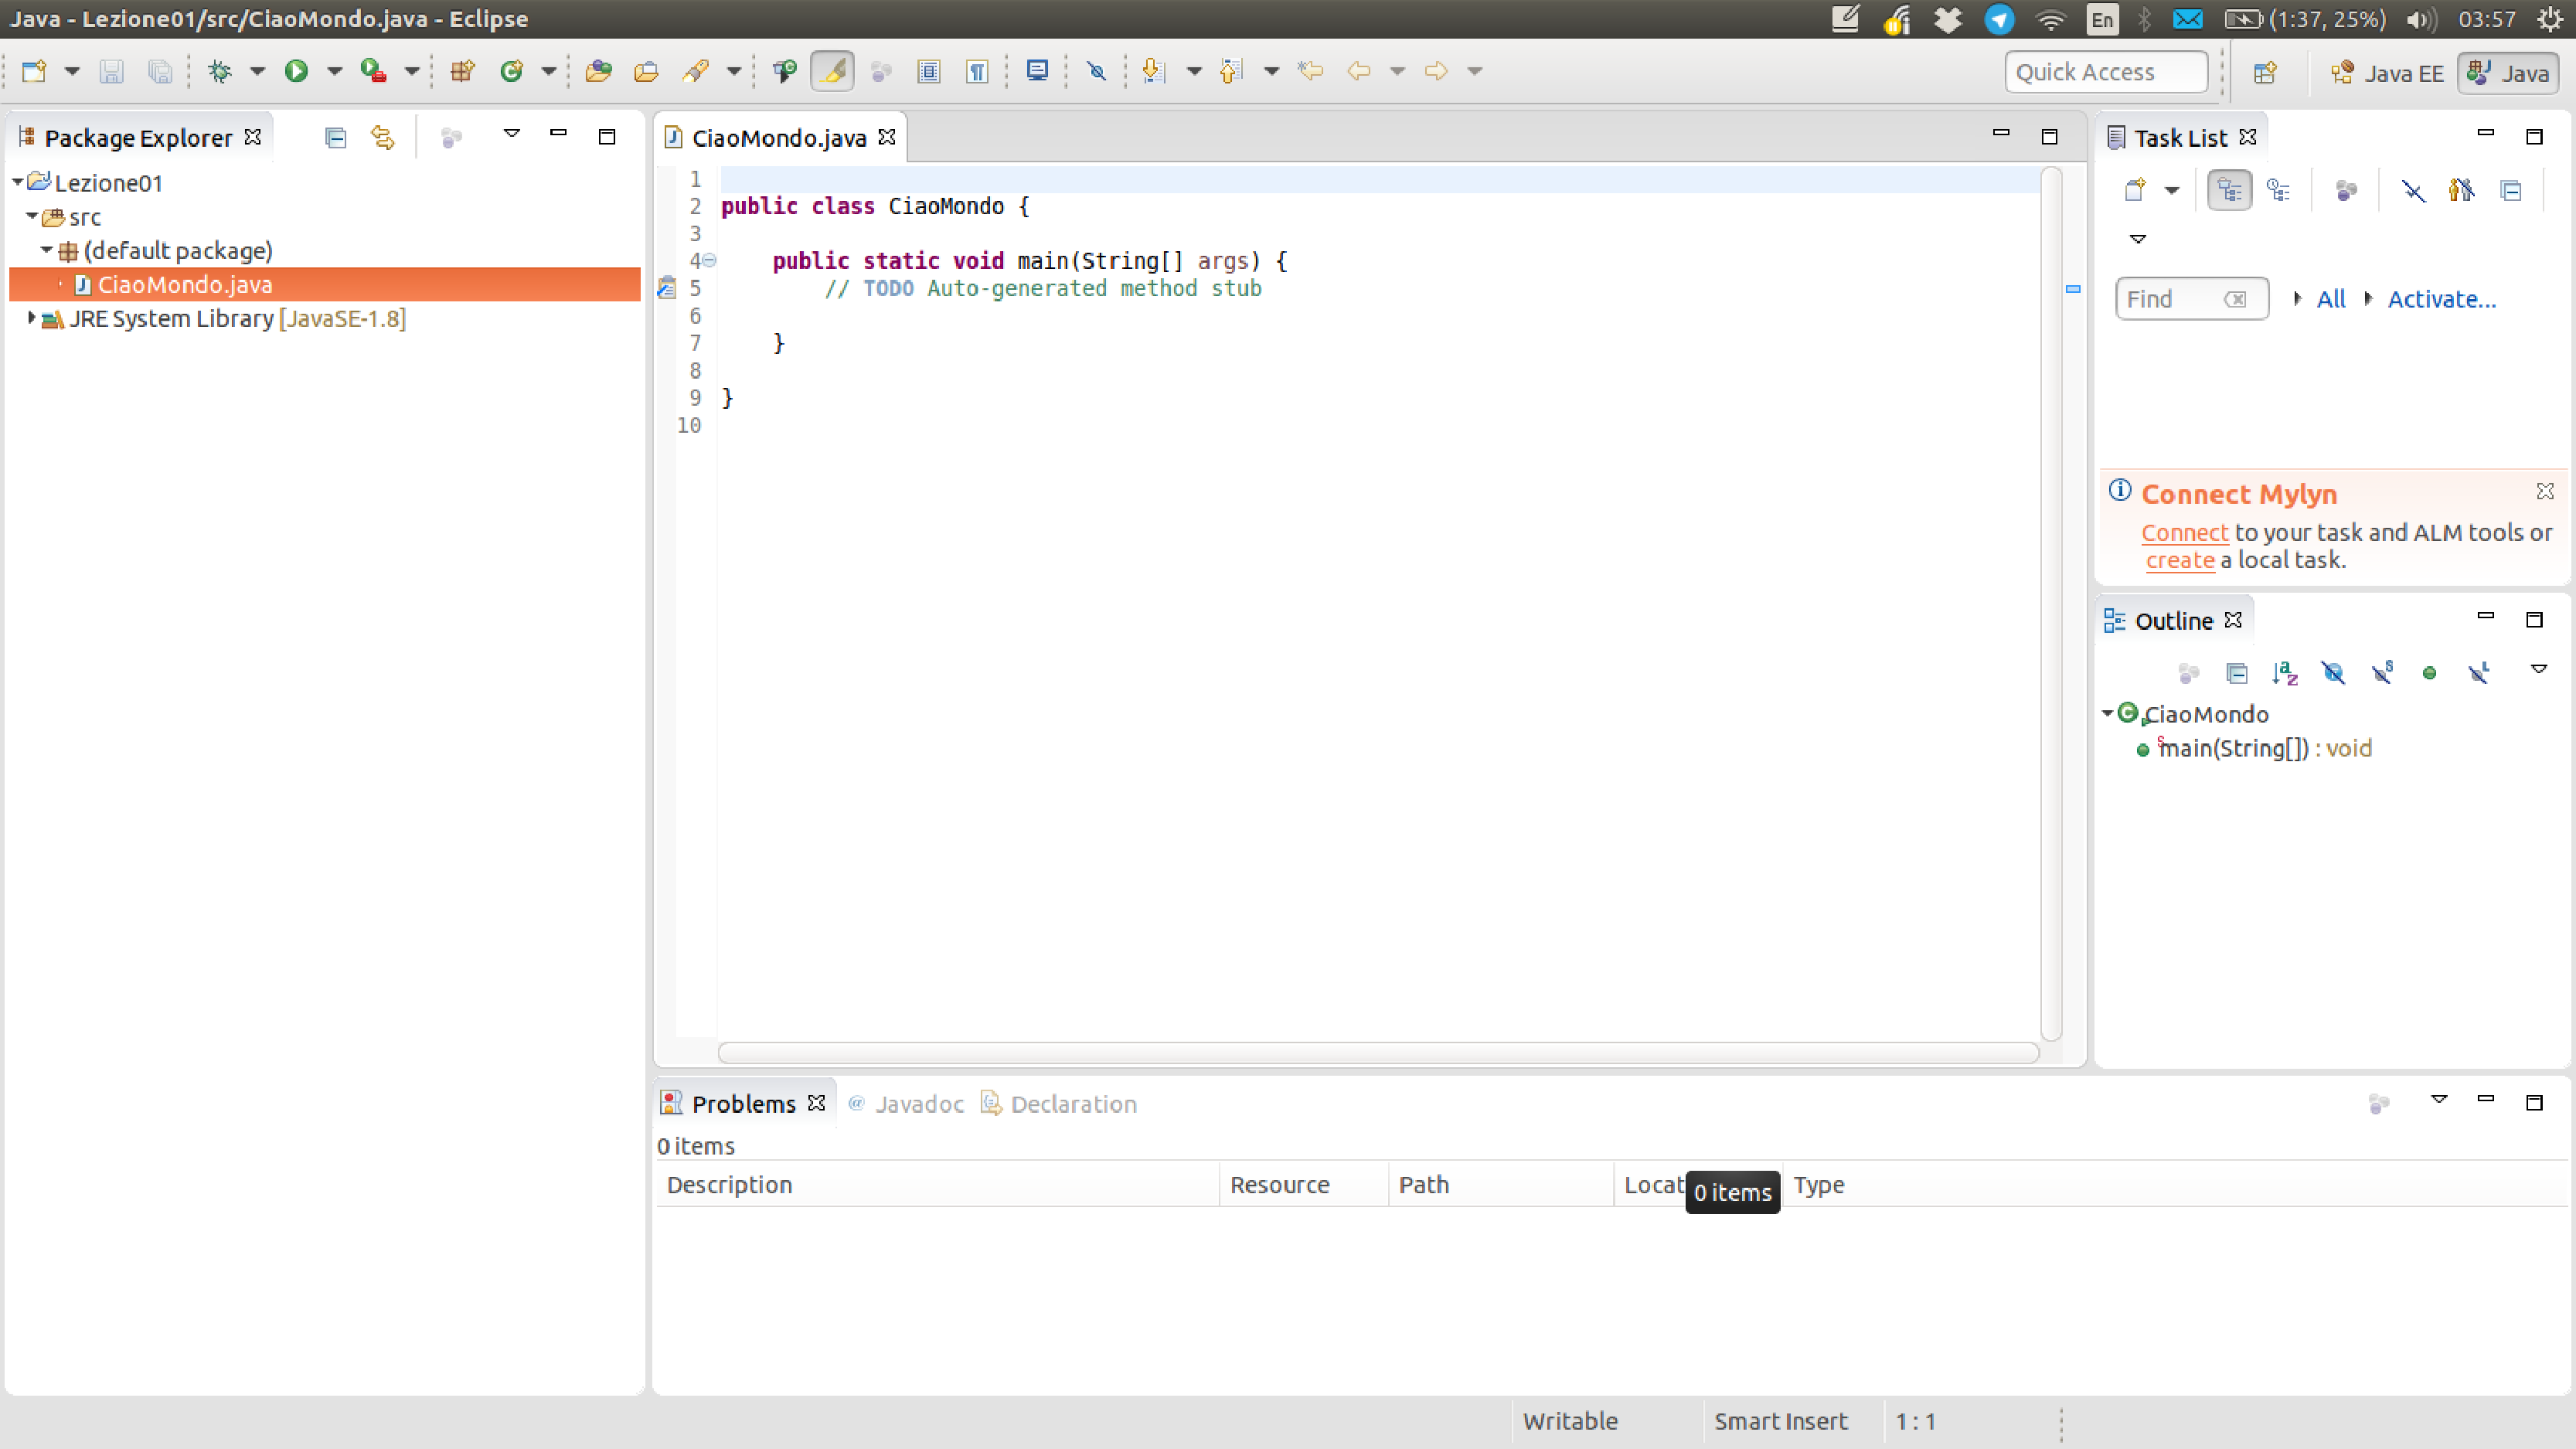
\includepdf[pages={1}]{img/eclipse/class_created.pdf}
}

% \pgfdeclareimage[height=\paperheight,width=\paperwidth]{code}{img/eclipse/code.png}
% \begin{frame}{Avvio di Eclipse}
%   \begin{center}
%     \pgfuseimage{code}
%   \end{center}
% \end{frame}
{
  \setbeamercolor{background canvas}{bg=}
  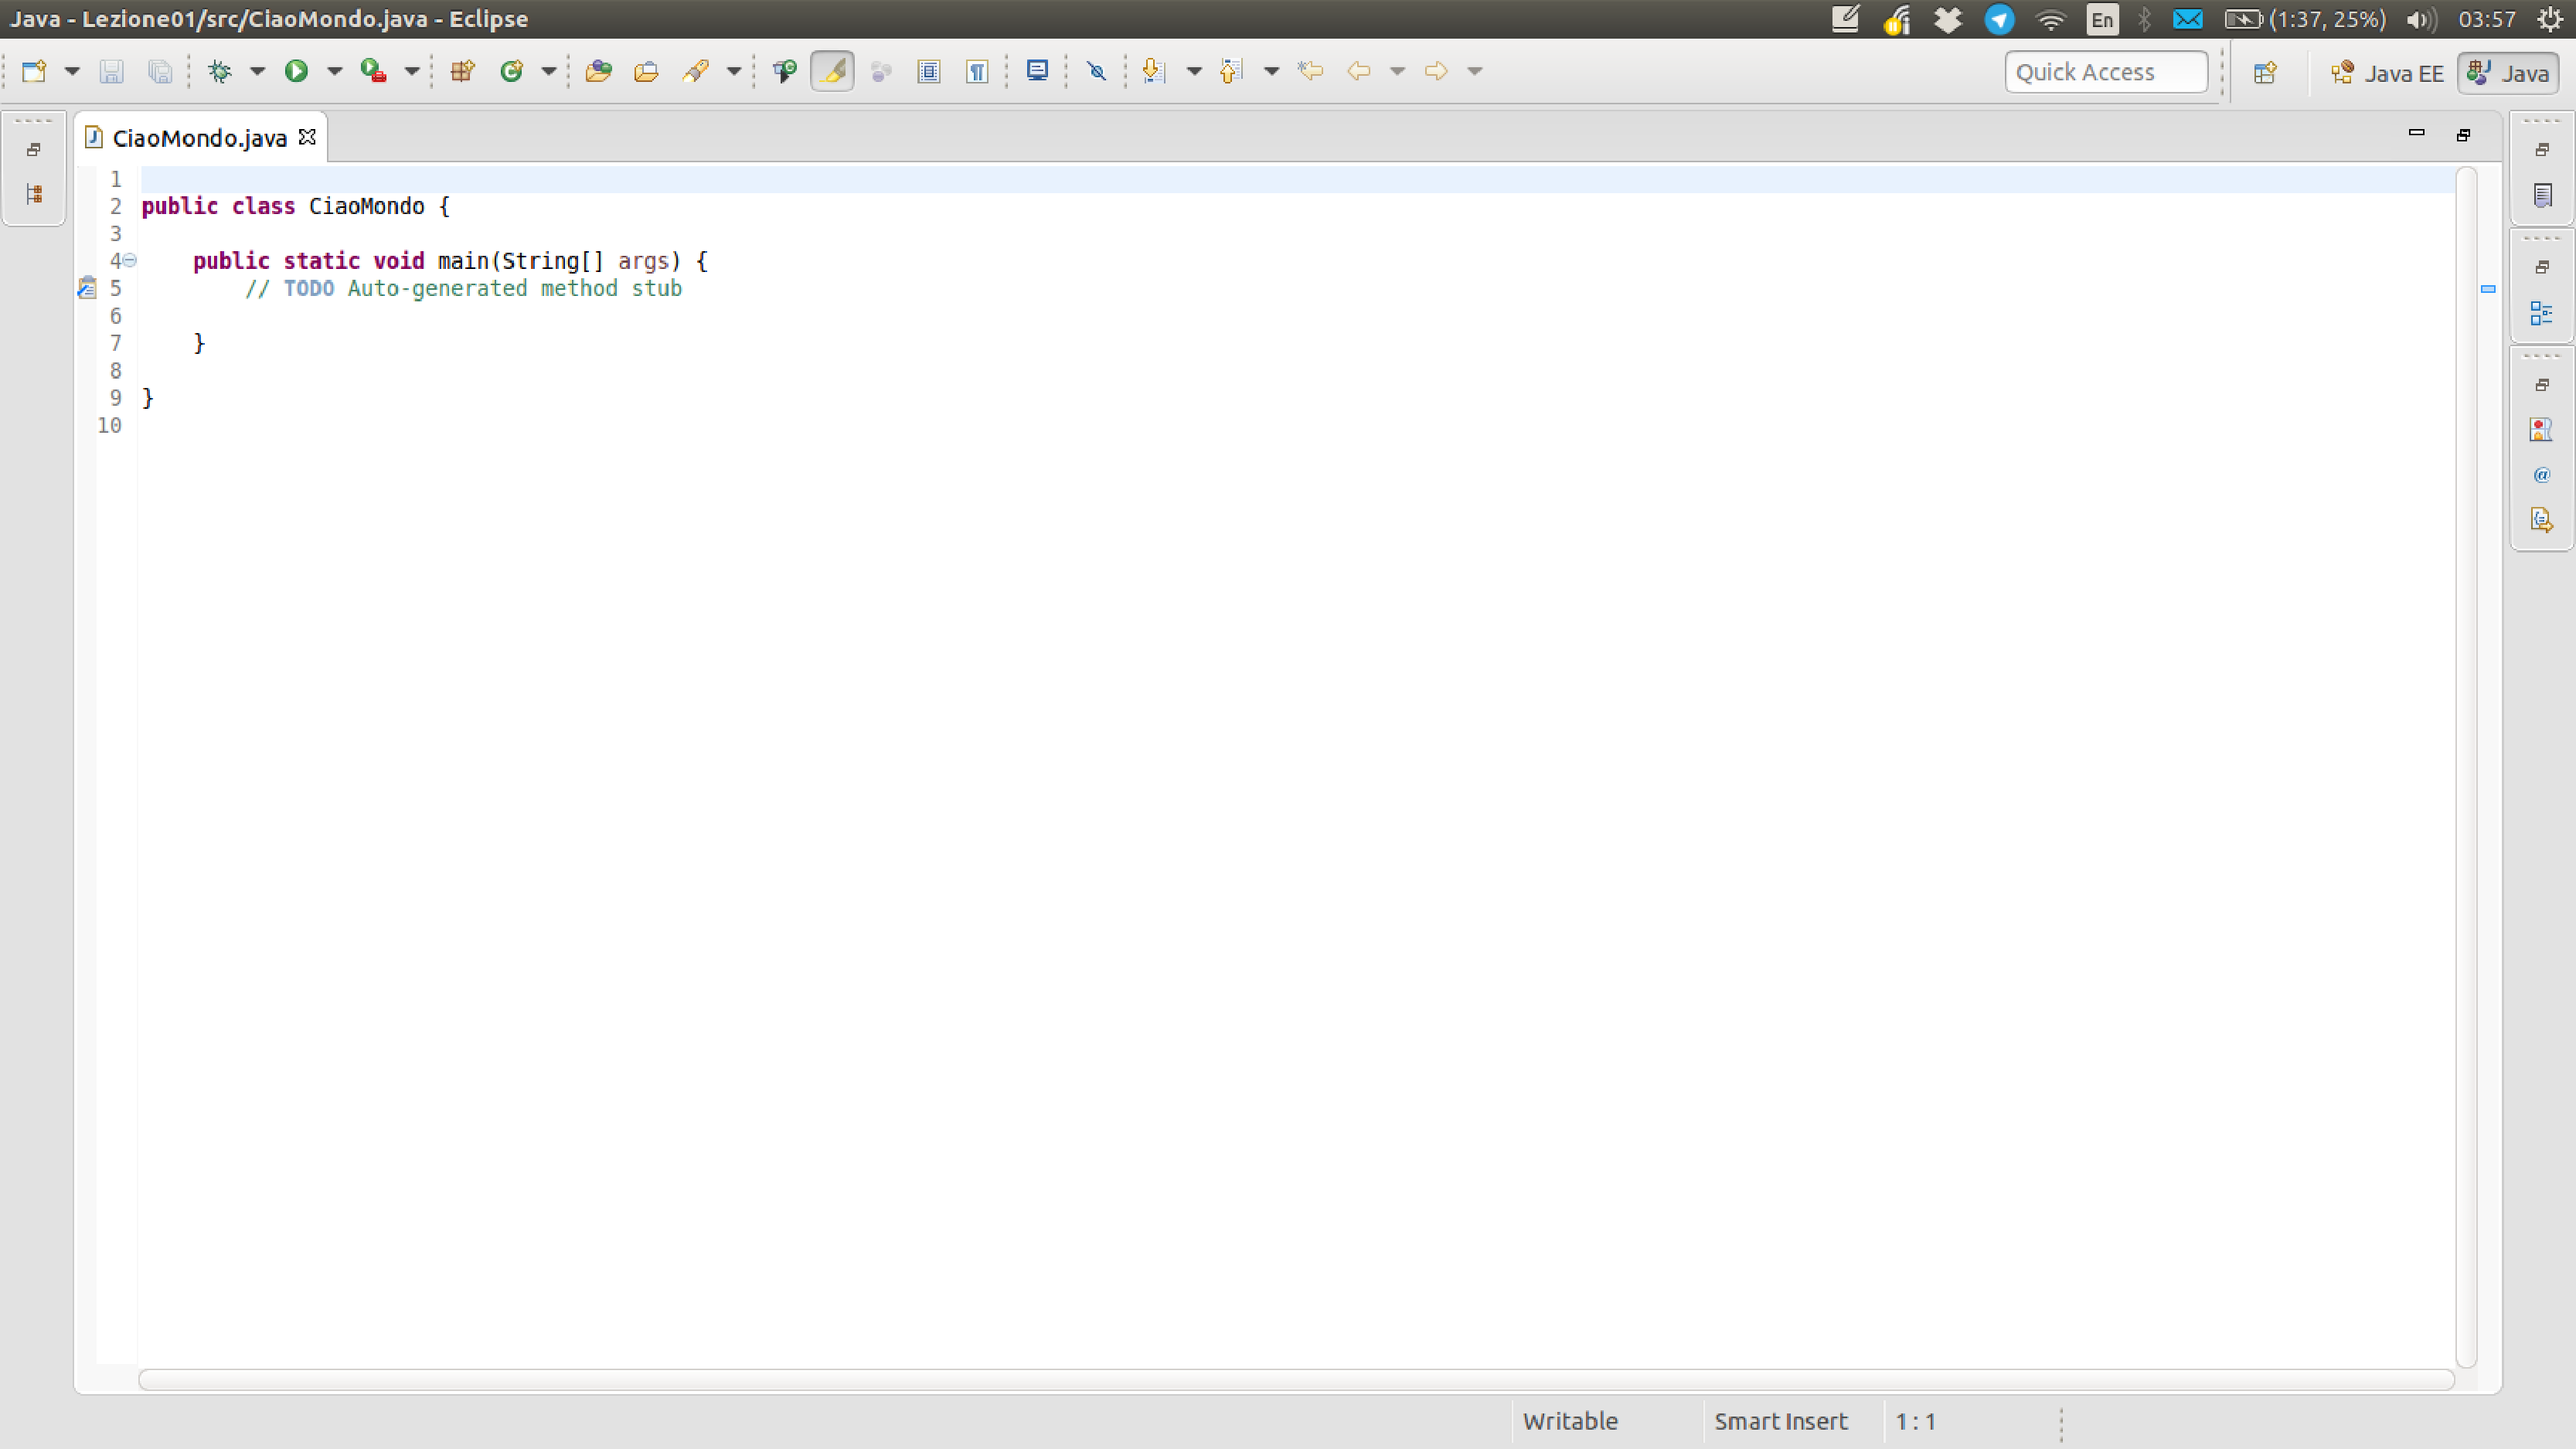
\includepdf[pages={1}]{img/eclipse/code.pdf}
}

% \pgfdeclareimage[height=\paperheight,width=\paperwidth]{suggestion}{img/eclipse/suggestion.png}
% \begin{frame}{Avvio di Eclipse}
%   \begin{center}
%     \pgfuseimage{suggestion}
%   \end{center}
% \end{frame}
{
  \setbeamercolor{background canvas}{bg=}
  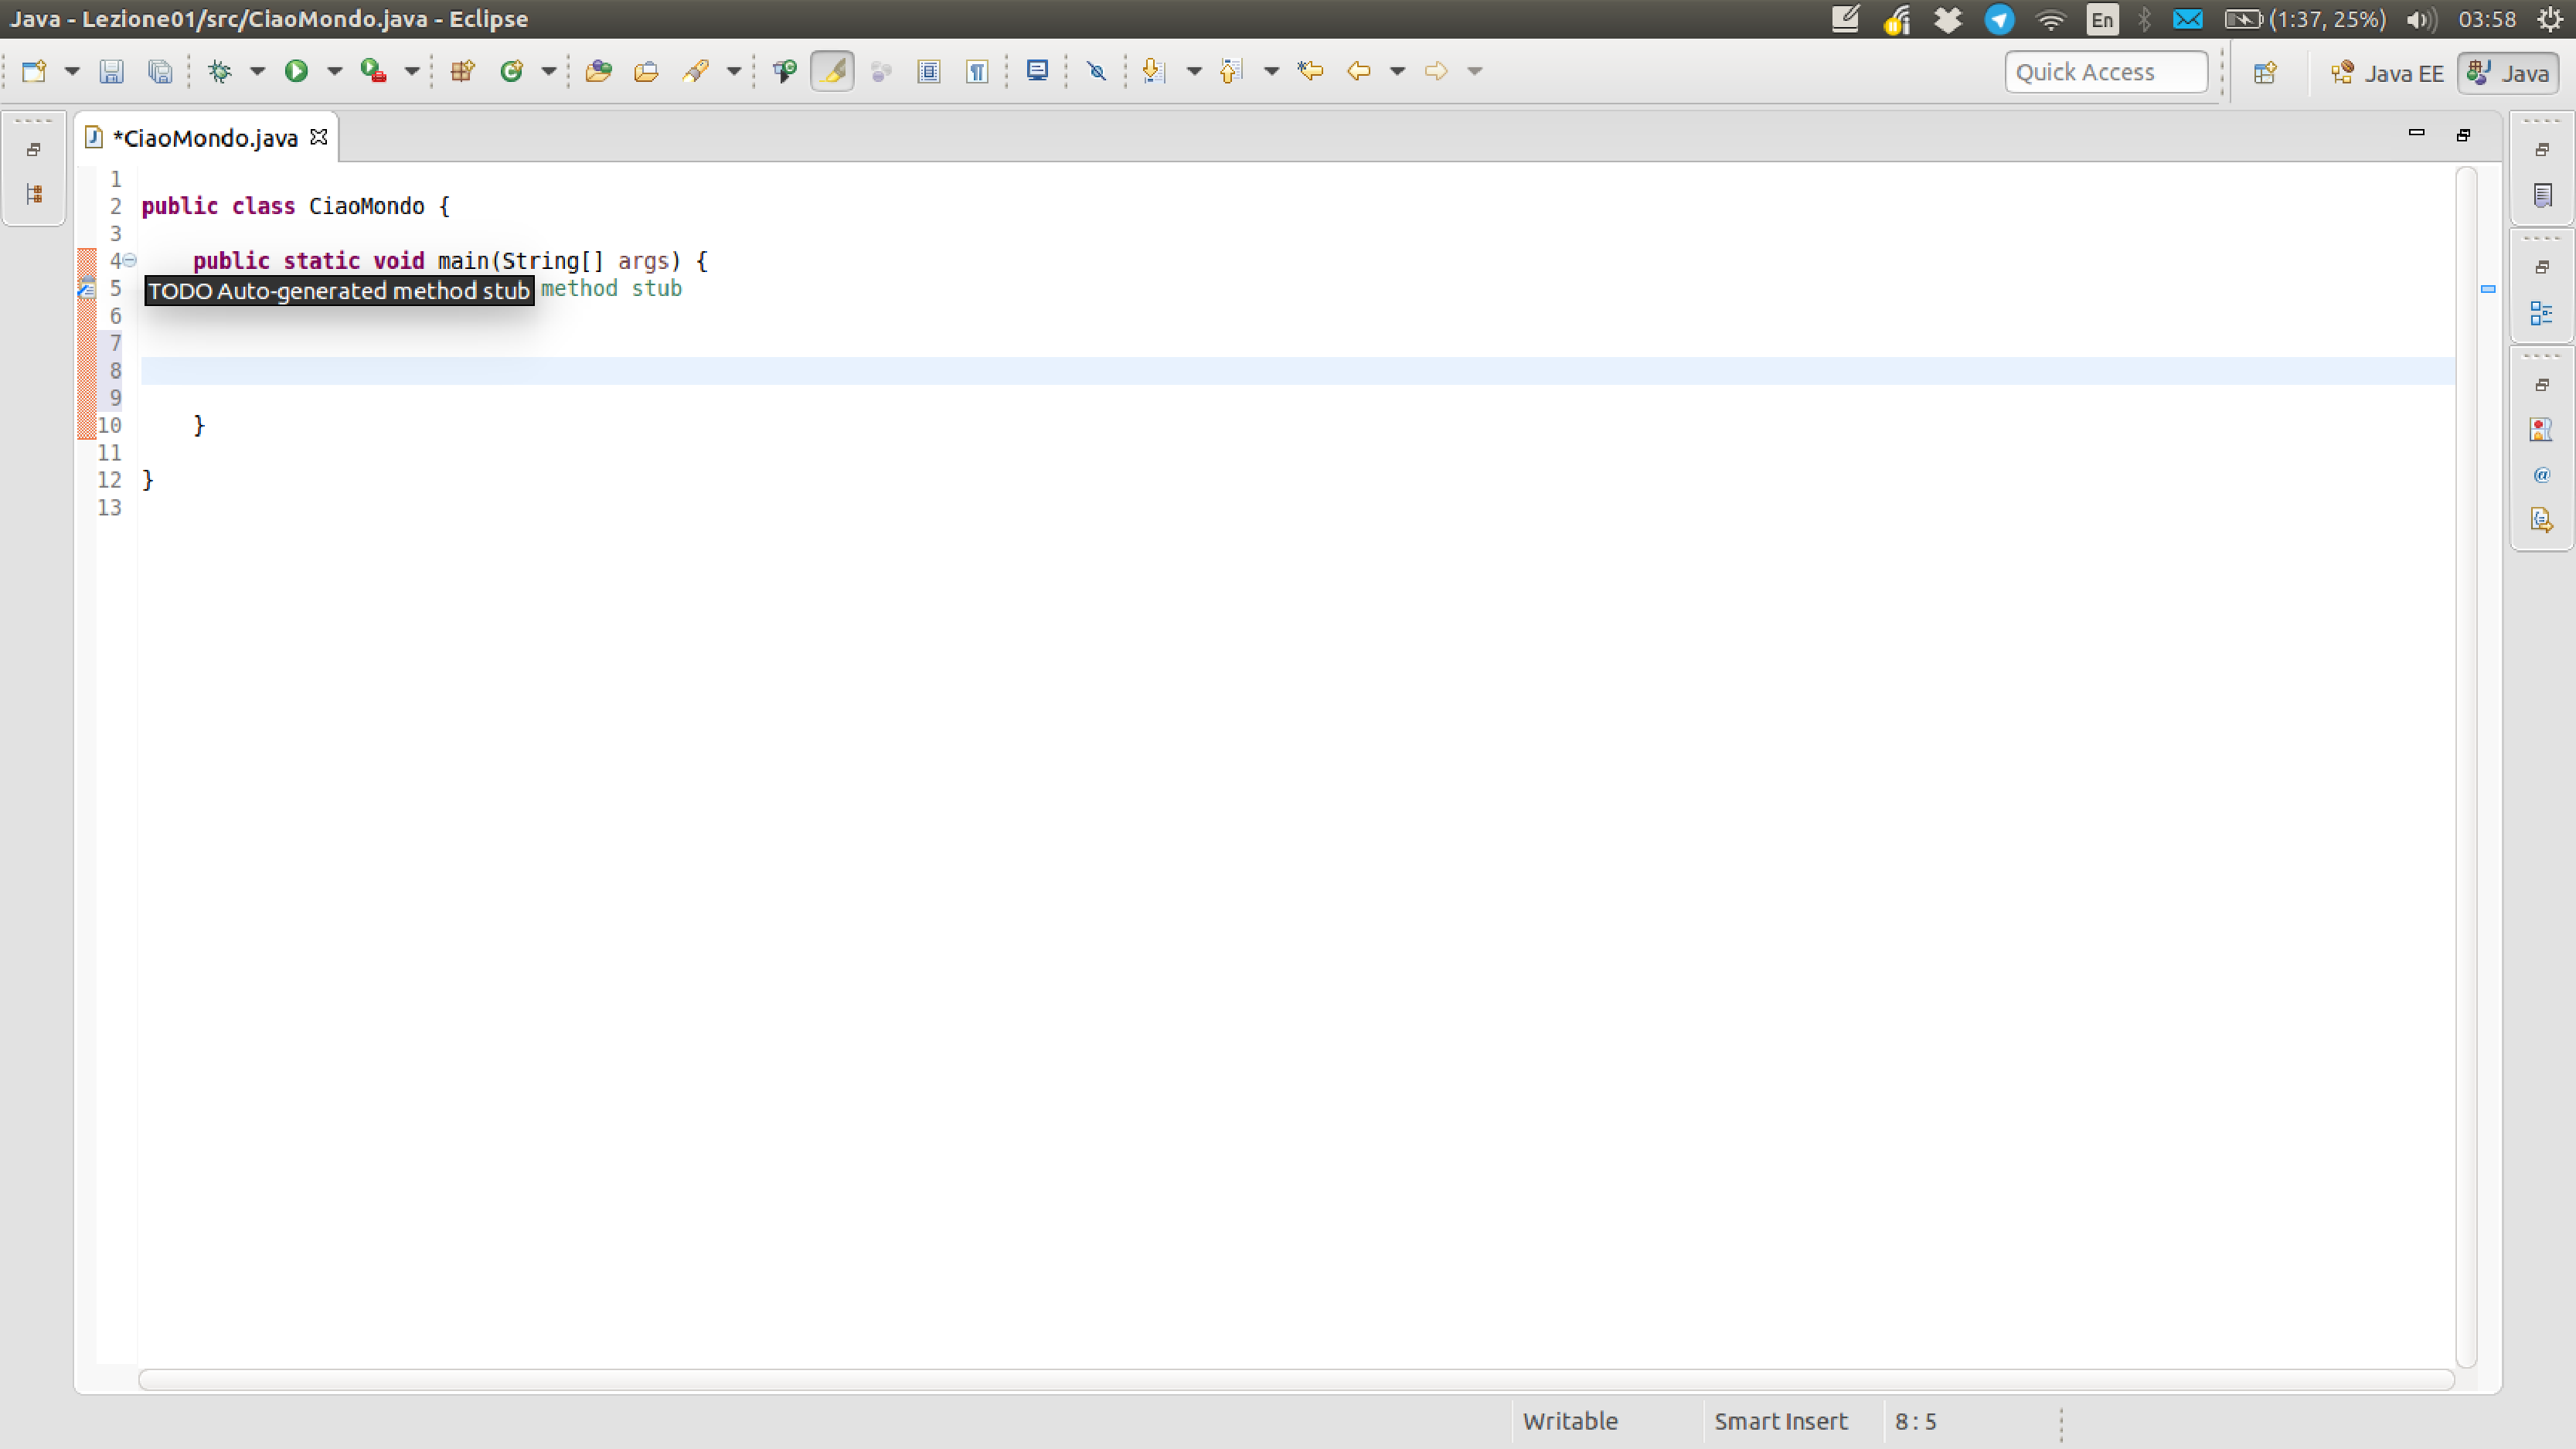
\includepdf[pages={1}]{img/eclipse/suggestion.pdf}
}

\pgfdeclareimage[width=0.5\paperwidth]{big_block}{img/big_block.png}
\begin{frame}{Blocchi (I)}
  \begin{center}
    \pgfuseimage{big_block}
  \end{center}
\end{frame}

\pgfdeclareimage[width=0.5\paperwidth]{big_block_code}{img/big_block_code.png}
\begin{frame}{Blocchi (II)}
  \begin{center}
    \pgfuseimage{big_block_code}
  \end{center}
\end{frame}